\providecommand{\main}{..}
\documentclass[\main/main.tex]{subfiles}

\begin{document}
\graphicspath{{img/}{06_result/img/}}

\chapter{System evaluation}

\section{Whole system overview}
\begin{figure}[H]
    \centering
    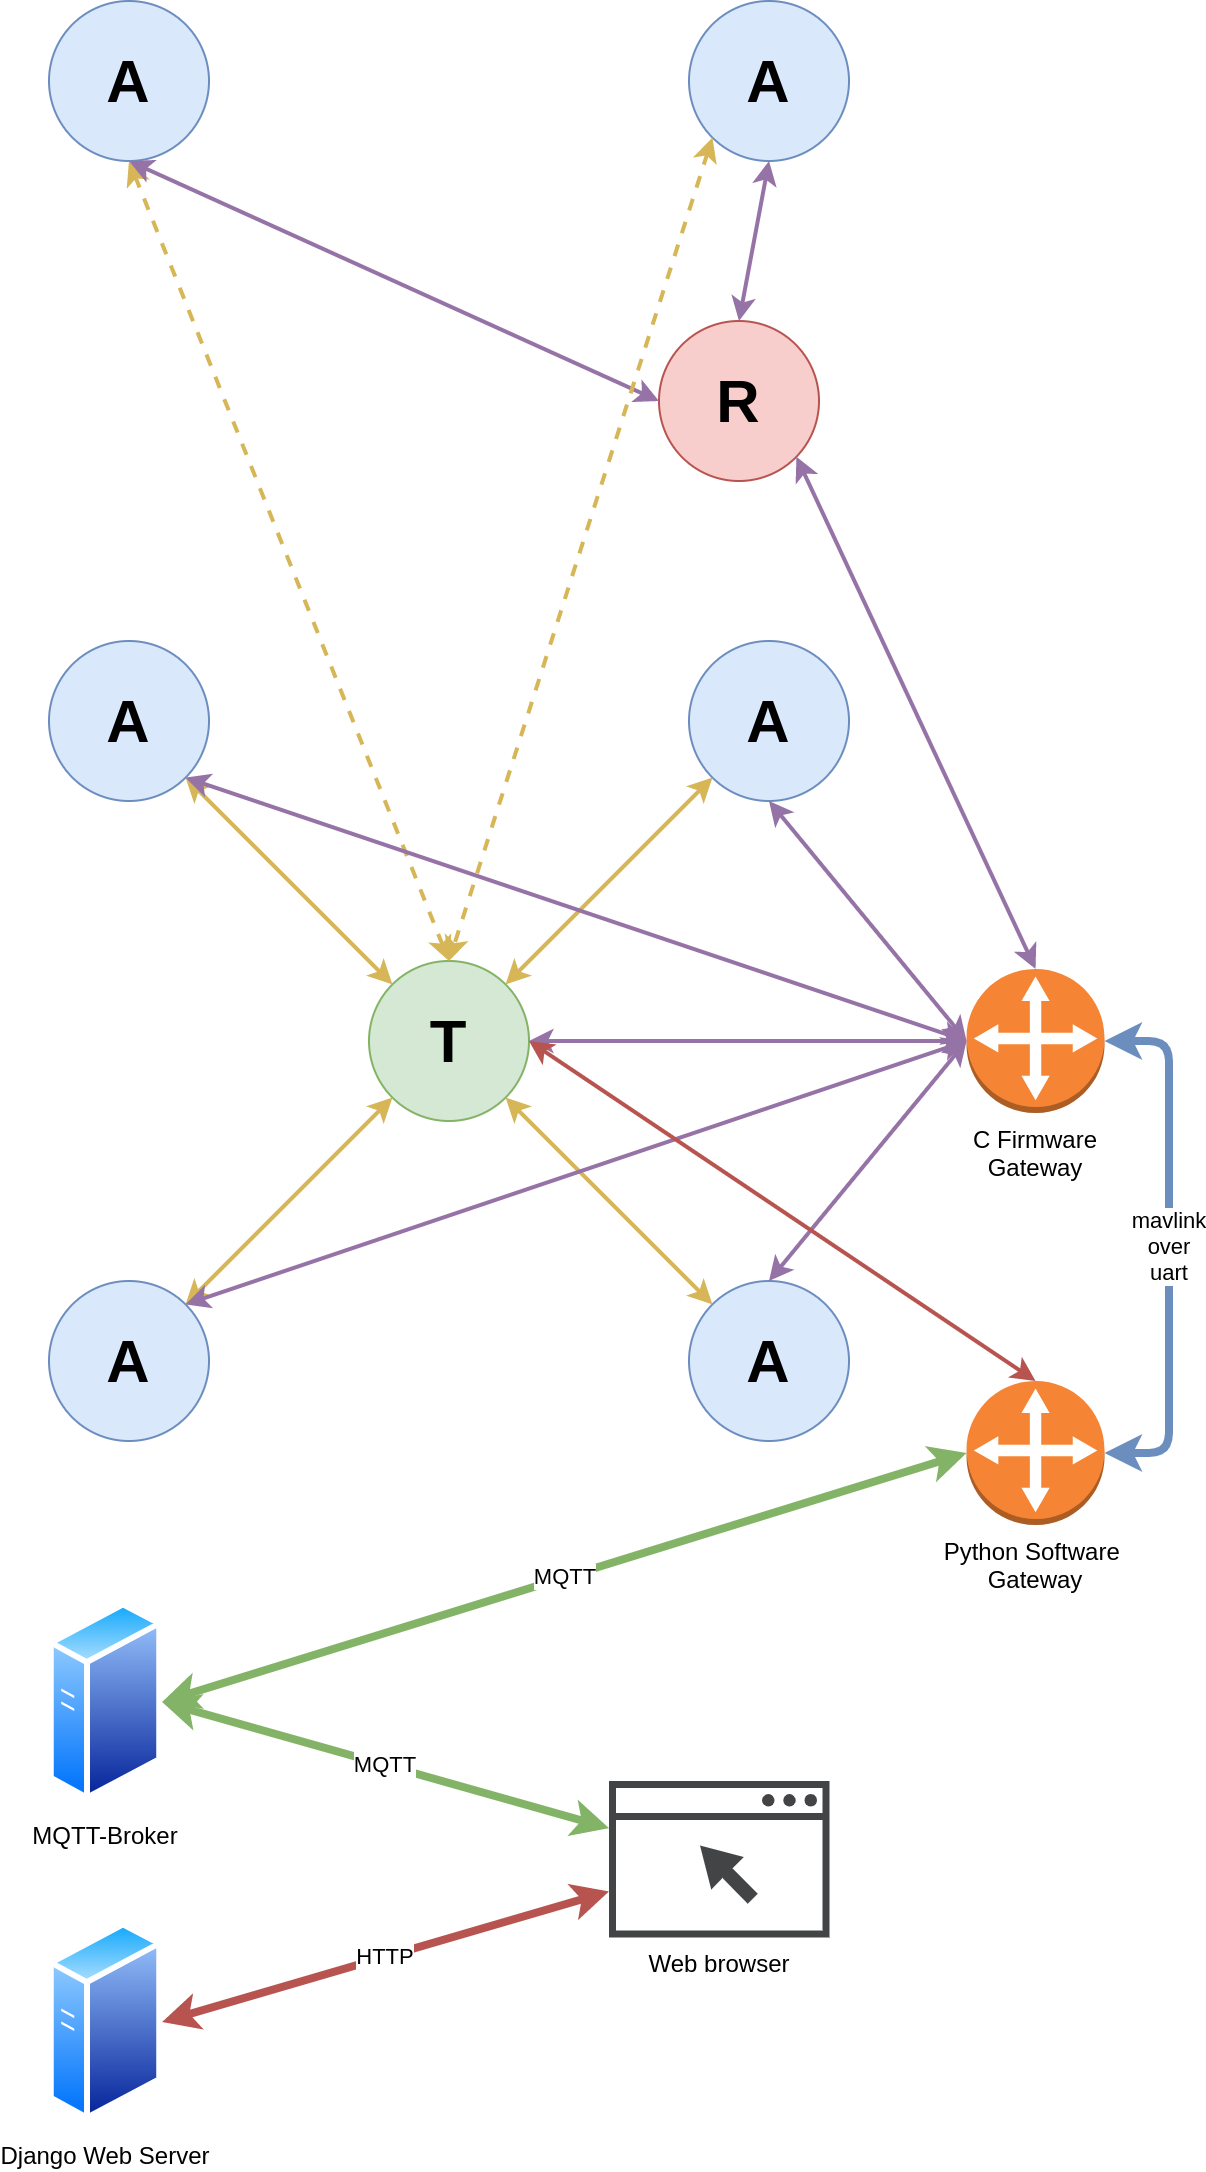
\includegraphics[width=0.9\textwidth]{system_overview.png}
    \caption{Whole system overview}
    \label{fig:system_overview}
\end{figure}
The whole system deployed in this thesis is illustrated in figure \ref{fig:system_overview}. There are three cells in the sample network and one tag located in each of the first two cells. Tags and anchors communicate with each other using 802.15.4 protocol over UWB radio. They, however, exchange messages with a gateway through a Bluetooth mesh network. The role of the relay node is to relay Bluetooth mesh messages as the distance between anchors/tags and gateway may longer than the effective communication range of Bluetooth-based devices. The firmware and software part of the gateway internally communicate using MAVLink protocol over a UART connection. The MAVLink frame is then stringified to JSON format and published to an MQTT broker. The control and management system is a web-based application. A Django server provides web service for this application. When receiving an HTTP request from the browser, the Django server returns an HTML/CSS-based GUI (Graphic User Interface) together with instructions for the browser to connect to the MQTT broker. In this way, the browser subscribes to the right topic. On receiving event messages from the gateway, the browser processes and shows them on the screen in a programmed way. On receiving controls from users, the browser publishes the corresponsive JSON messages to a specific topic that has been already subscribed by the gateway. The gateway then passes such messages to the mesh network.

\section{Evaluation}

In all experiments, the location error is calculated follow equation \ref{eqn:root_mean_square}.
\begin{equation}
    e_{RMS} = \frac{1}{n} \sum_{k=1}^{n} \sqrt{(x_k-x_{kg})^2 + (y_k-y_{kg})^2 + (z_k-z_{kg})^2}
    \label{eqn:root_mean_square}
\end{equation}

\subsection{Preparation}
This subsection provides images to illustrate the experimental setup used to evaluate the proposed localization system. The logical configuration of the system has been given in figure \ref{fig:system_overview}. The physical placement of devices is represented in figure \ref{fig:physical placement of devices}.

\begin{figure}[H]     
    \centering
    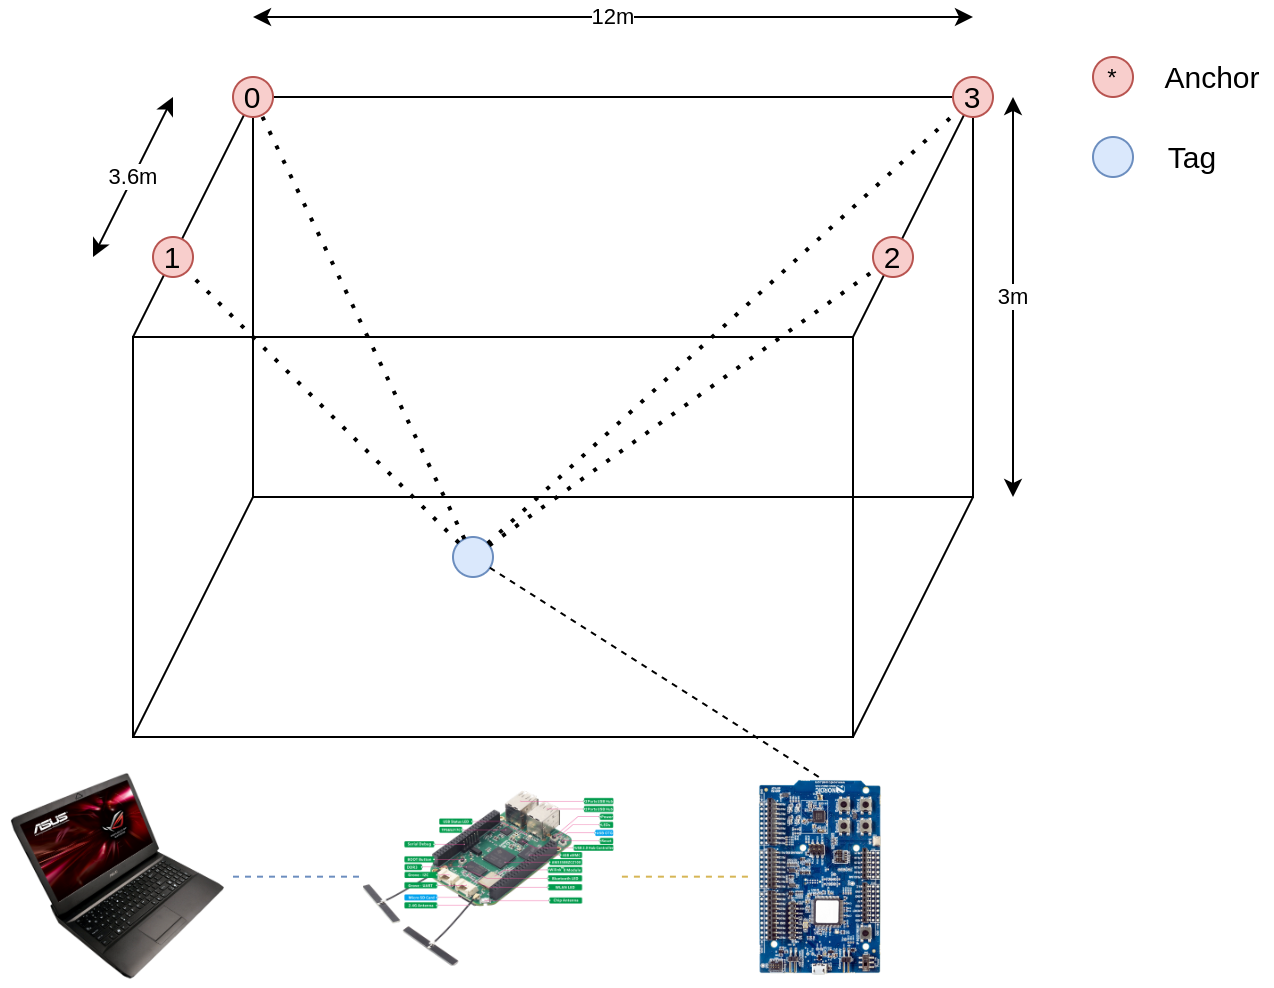
\includegraphics[width=0.9\textwidth]{system_overview_phy.png}
    \caption{Physical placement of devices}
    \label{fig:physical placement of devices}
\end{figure}
The actual placement of devices is shown in figures: \ref{fig:arena_00}, \ref{fig:node_0_1}, \ref{fig:node_2_3}, \ref{fig:node_4_5_6_7}.

\begin{figure}[H]      
    \centering
    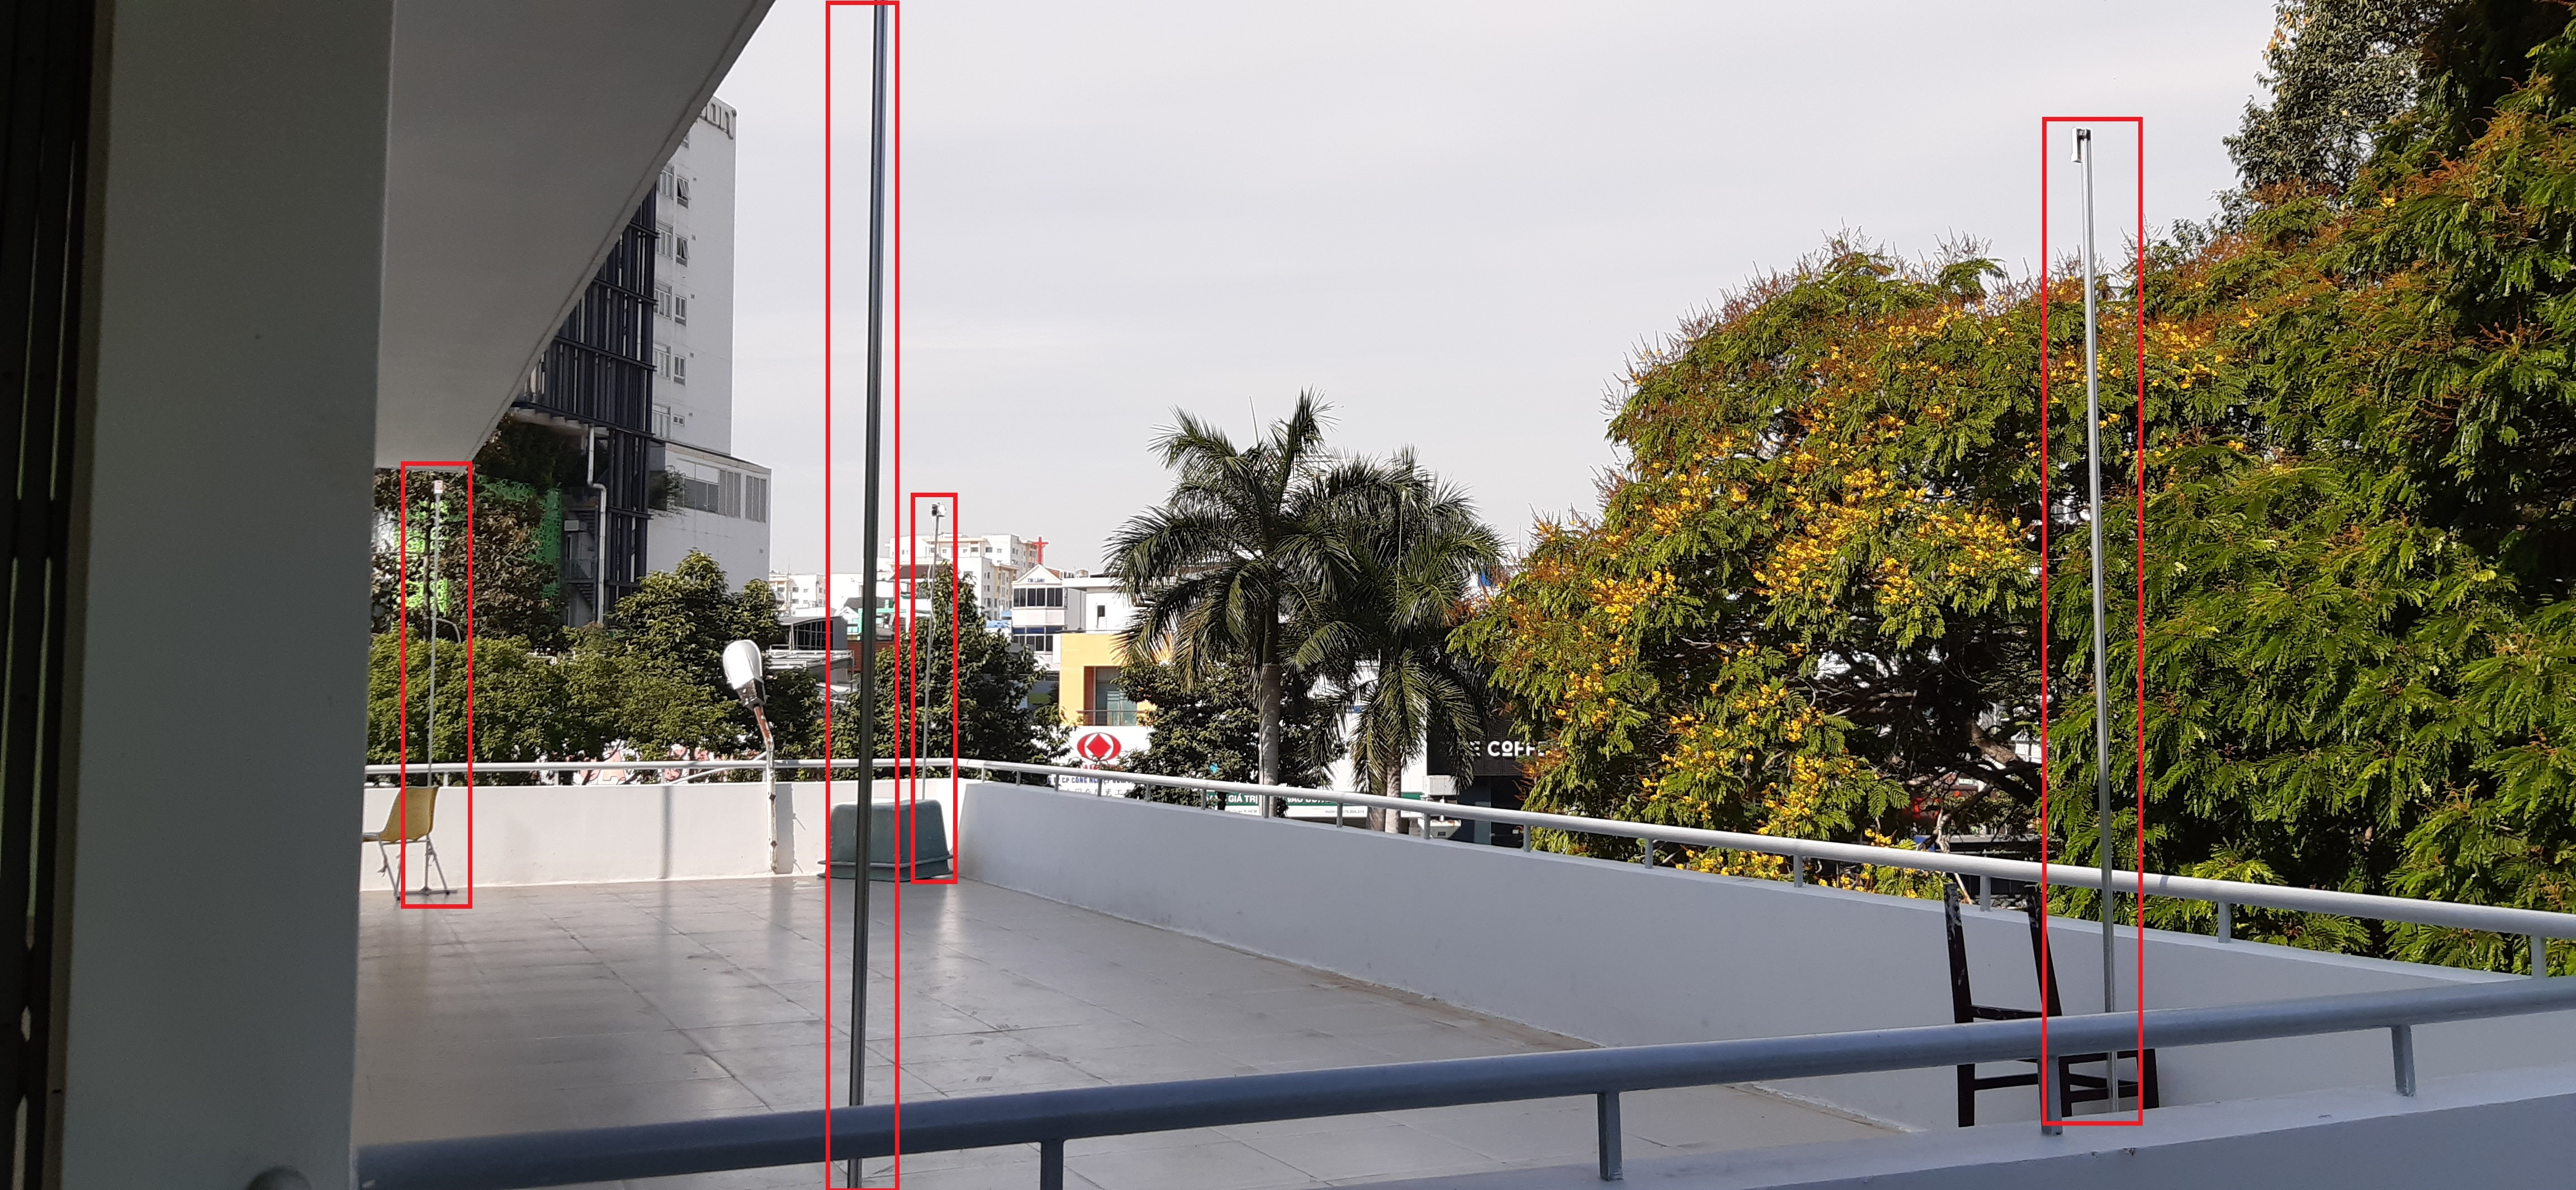
\includegraphics[width=1\textwidth]{arena_00.jpg}
    \caption{Arena side view}
    \label{fig:arena_00}
\end{figure}

% \begin{figure}[H]
%     \centering
%     \begin{subfigure}[b]{0.4\linewidth}
%         \centering
%         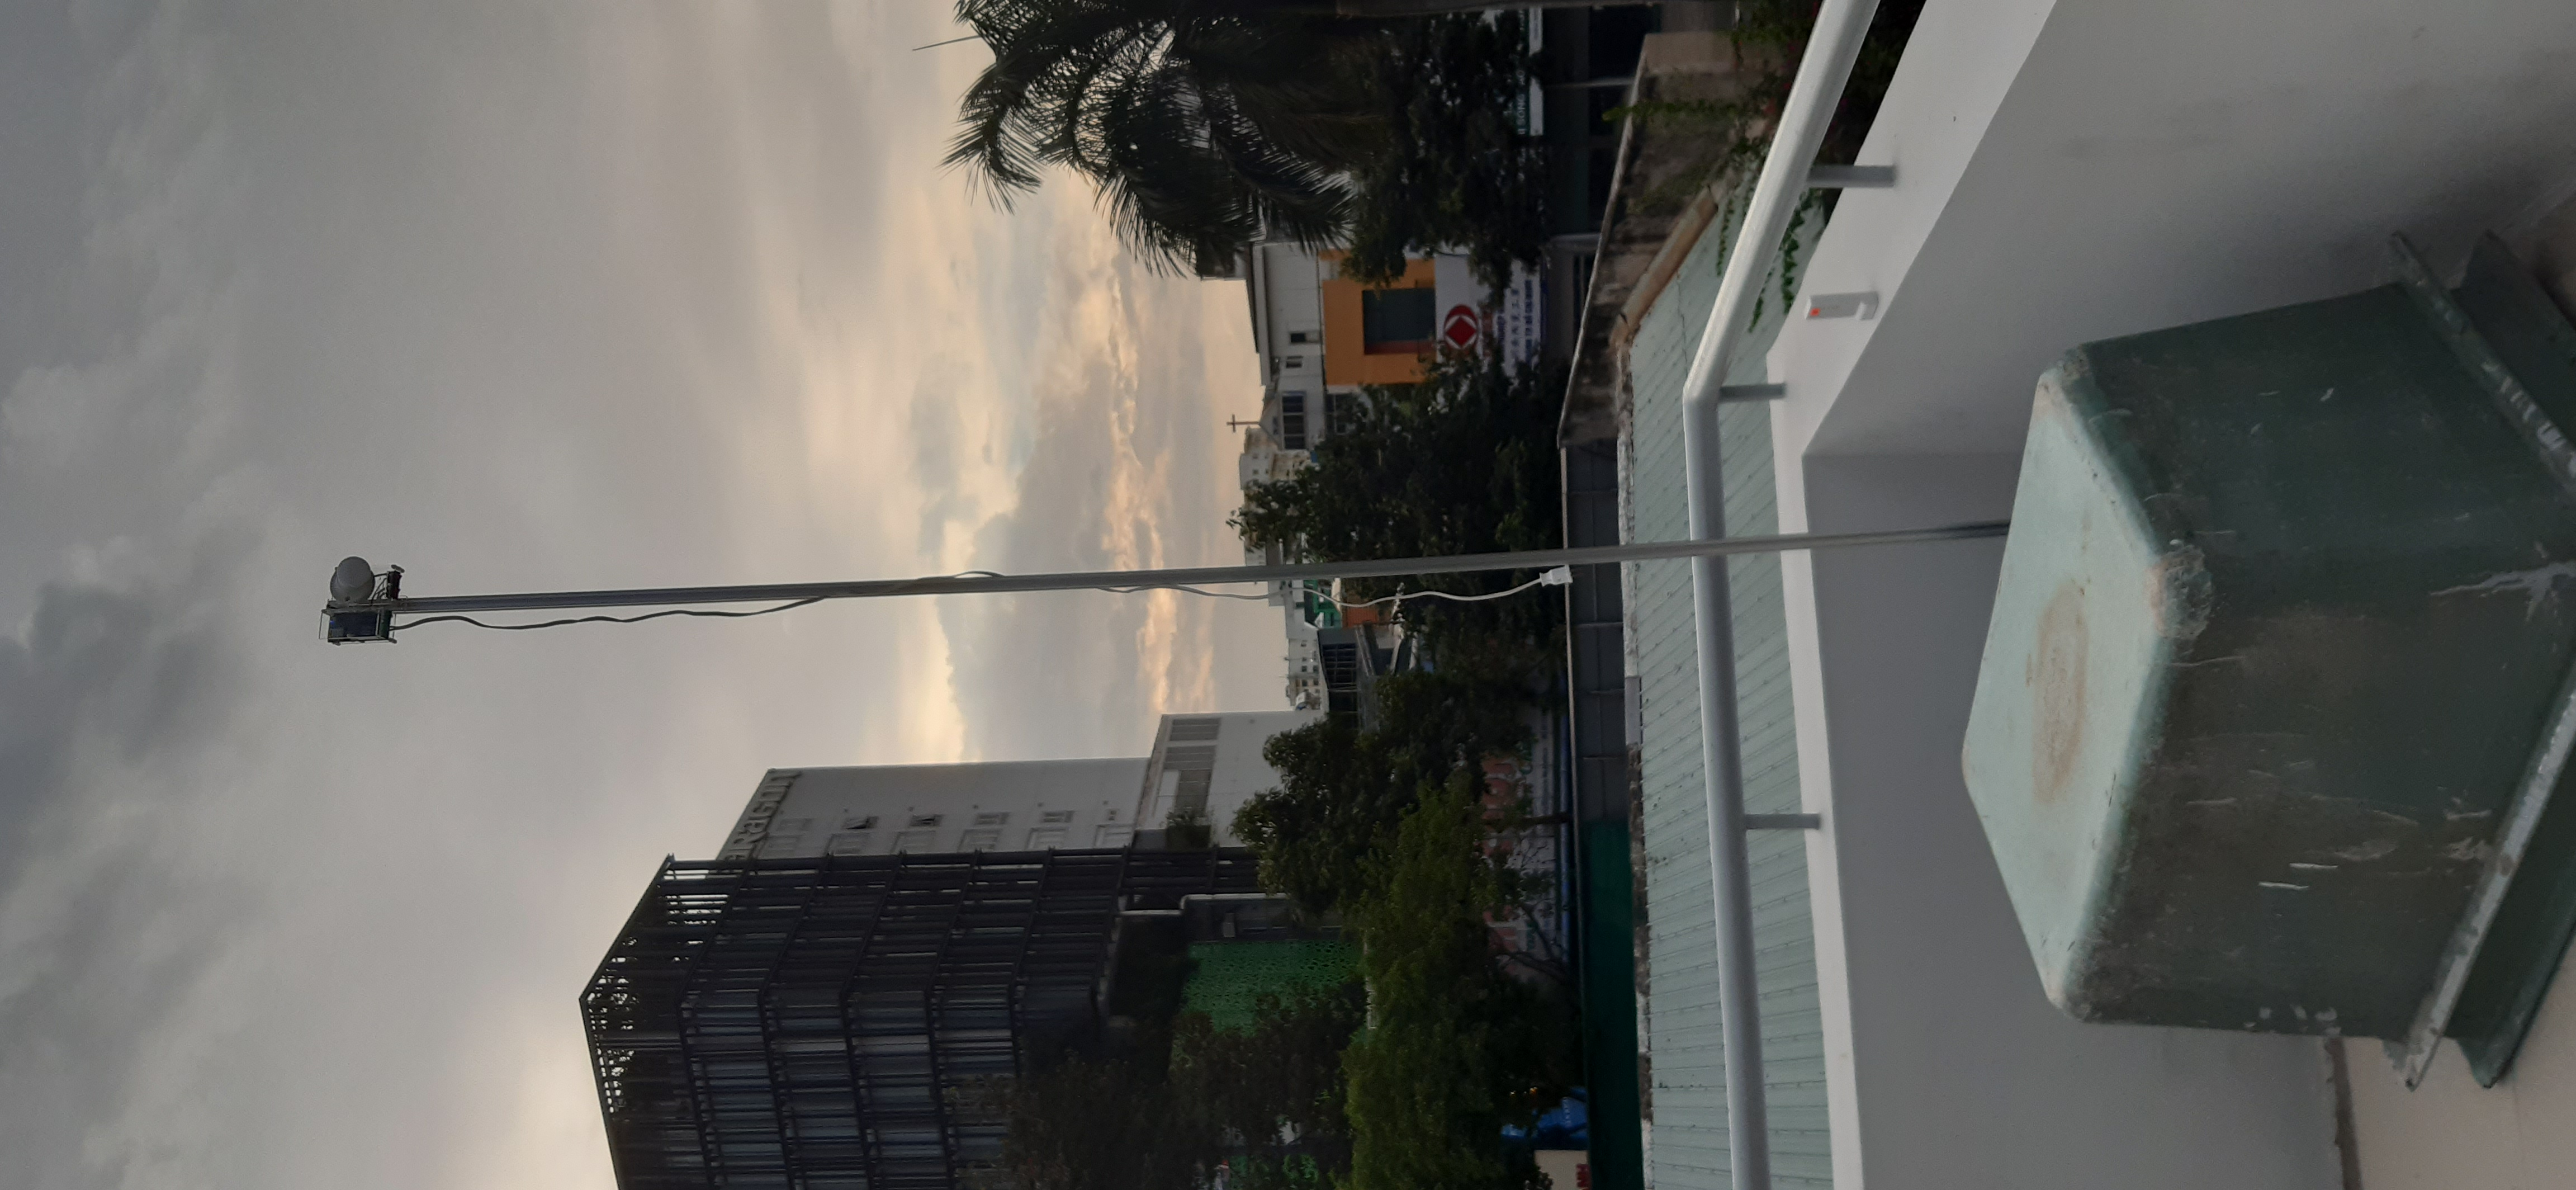
\includegraphics[angle=-90, width=0.65\linewidth]{arena_04.jpg}
%         \label{fig:arena_04}
%     \end{subfigure}
%     \begin{subfigure}[b]{0.4\linewidth}
%         \centering
%         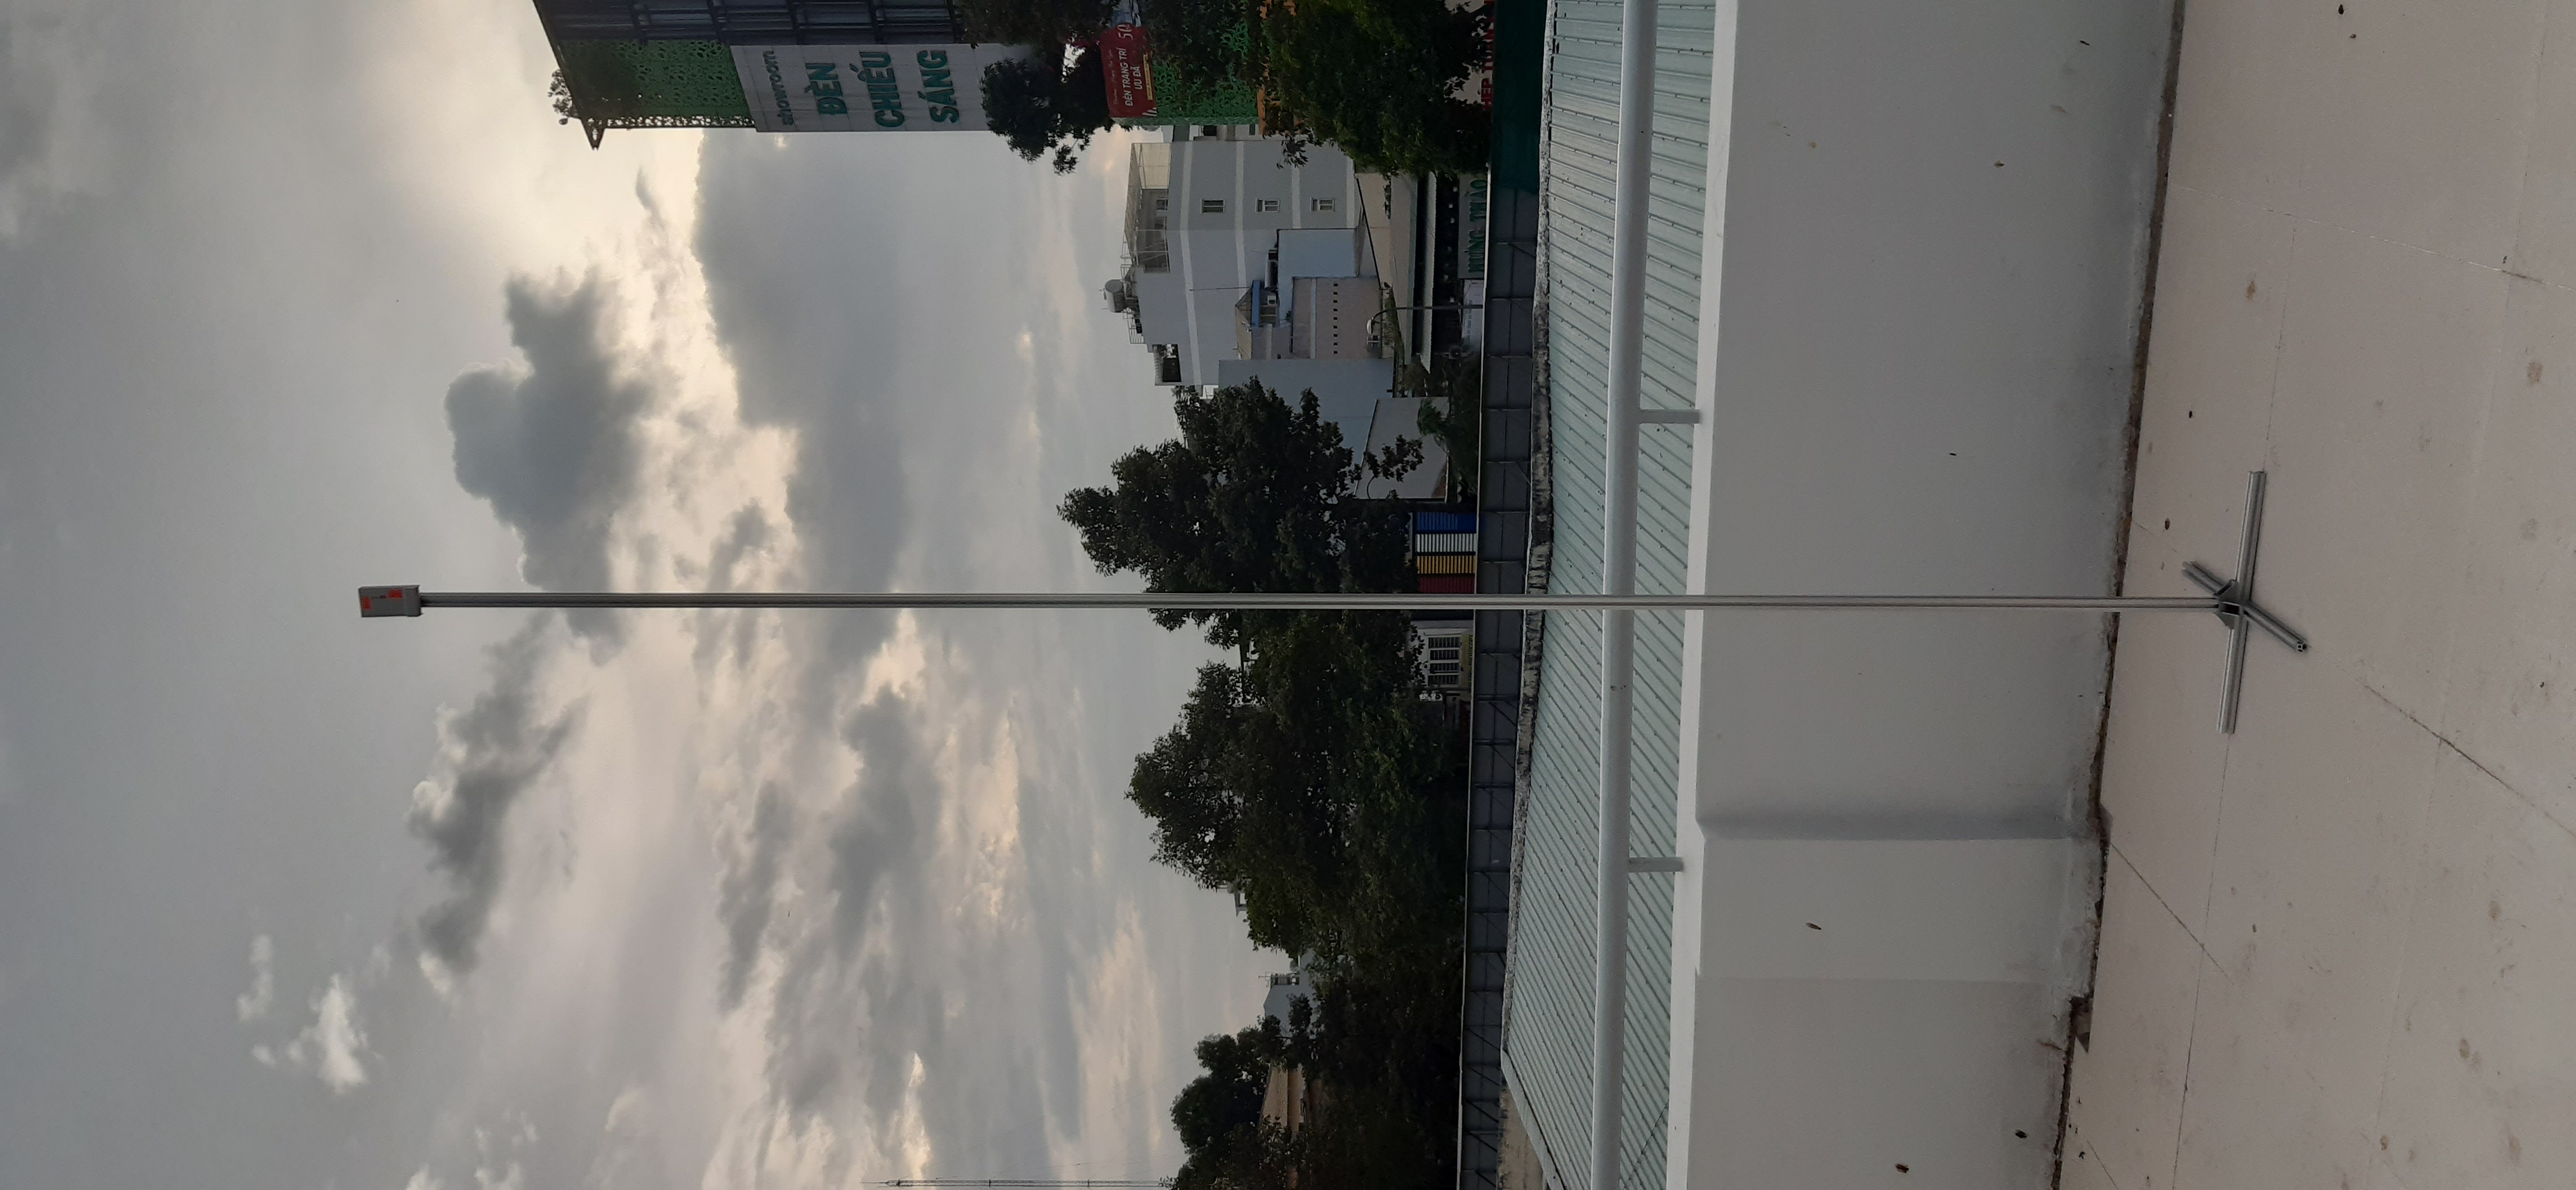
\includegraphics[angle=-90, width=0.65\linewidth]{arena_03.jpg}
%         \label{fig:arena_03}
%     \end{subfigure}
%     \caption{Node 0,1}
%     \label{fig:node_0_1_sep}
% \end{figure}

\begin{figure}[H]      
    \centering
    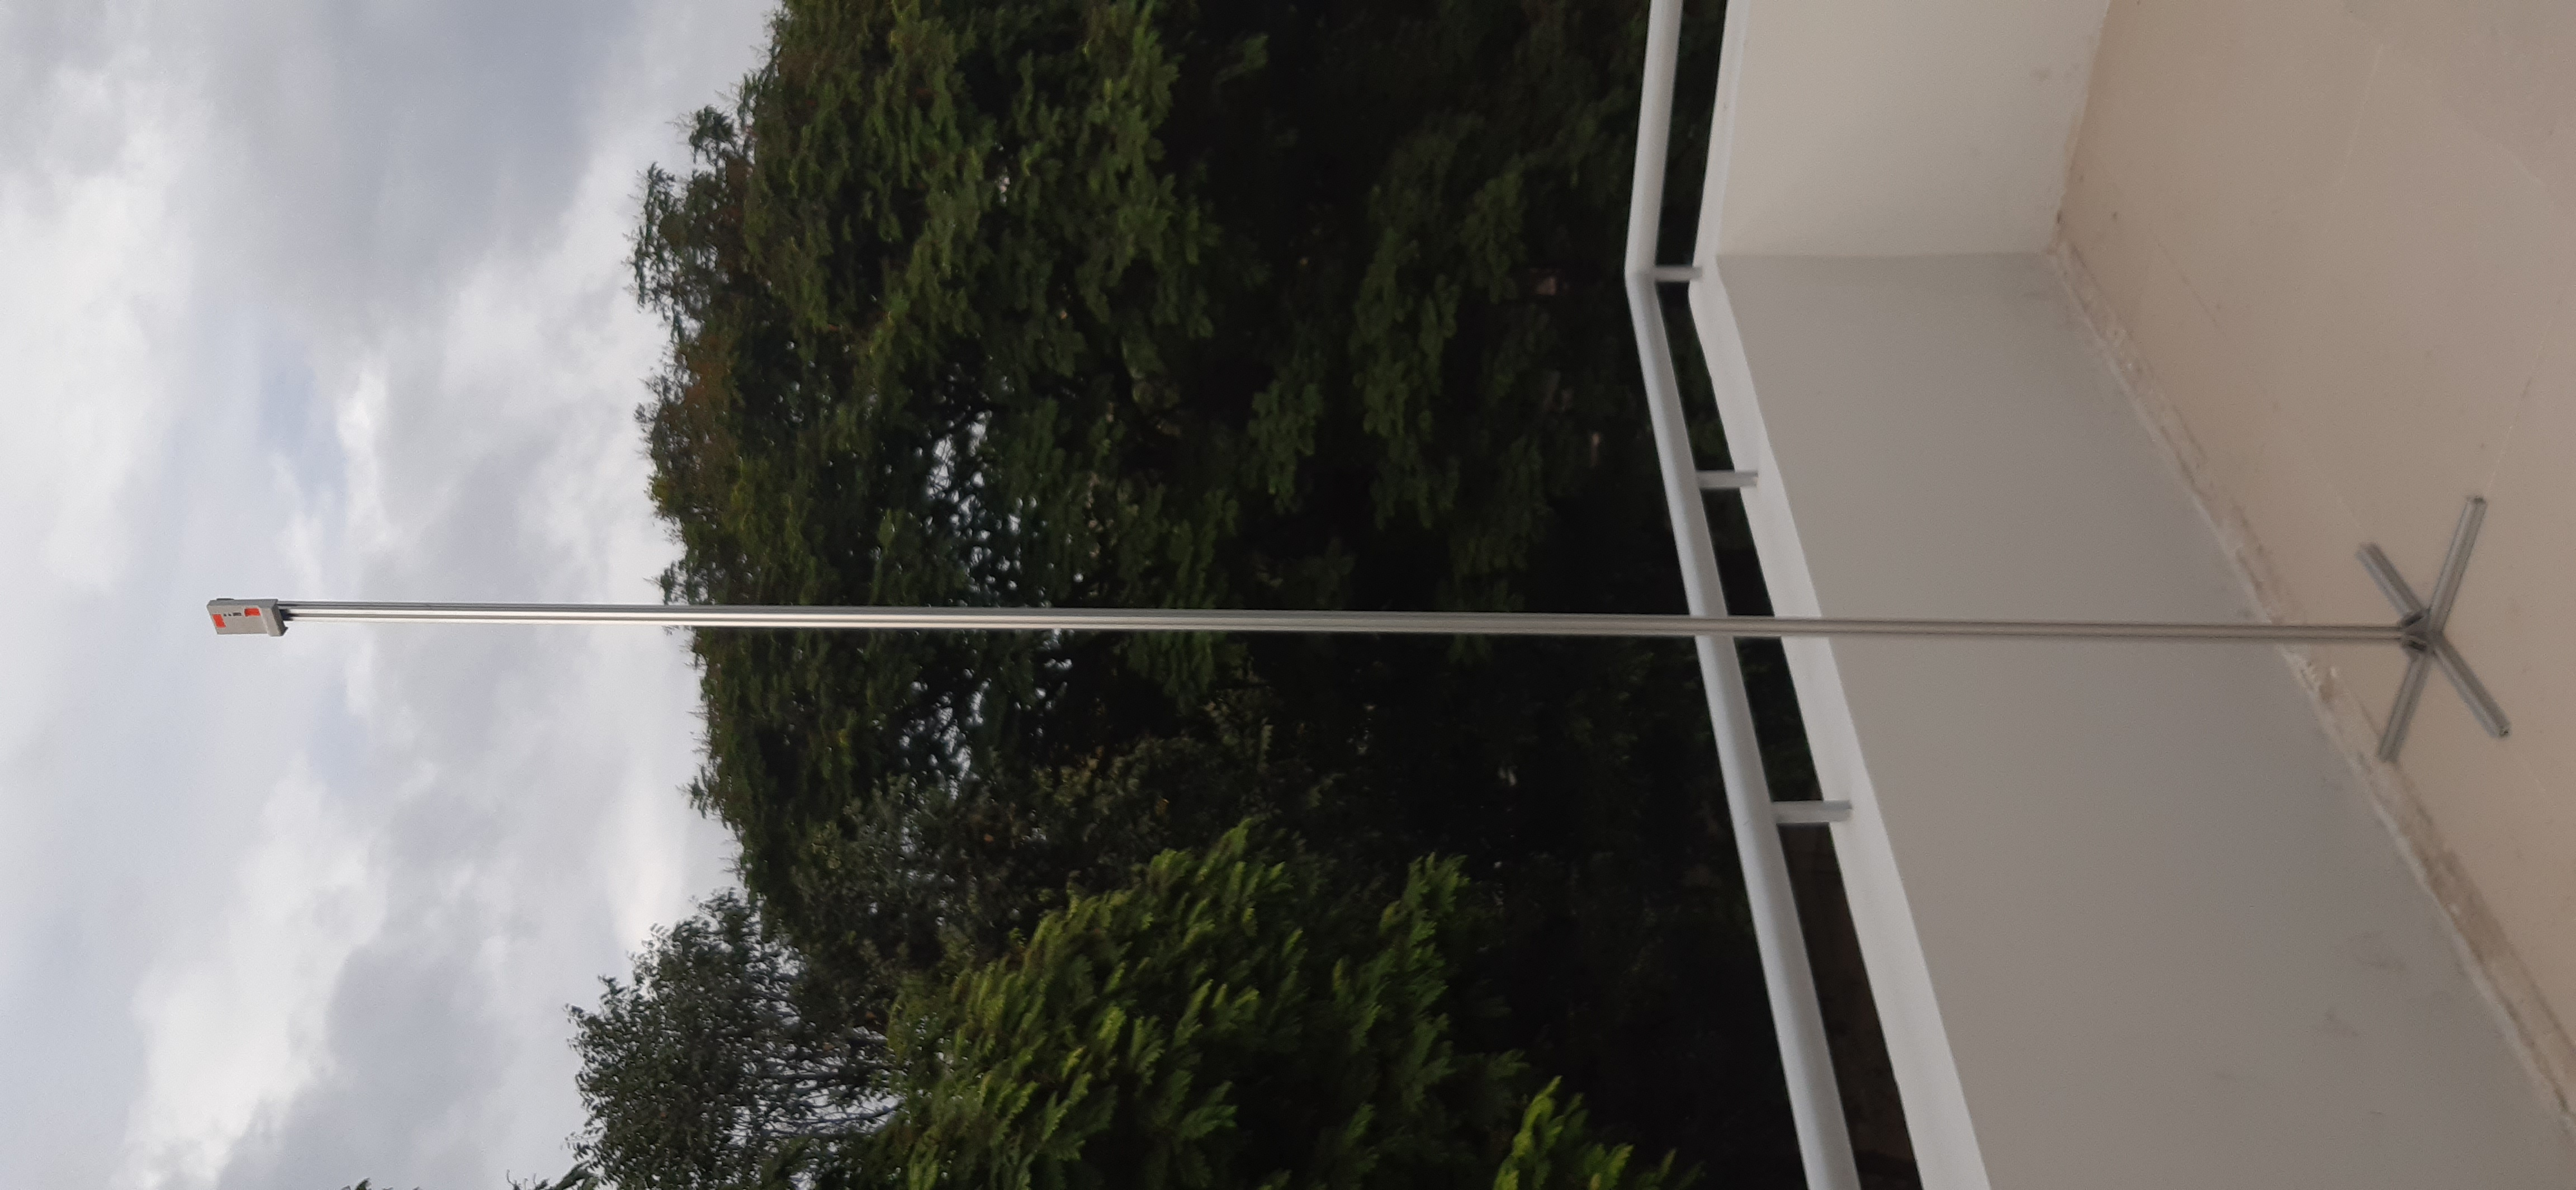
\includegraphics[width=1\textwidth]{arena_01.jpg}
    \caption{Node 0,1}
    \label{fig:node_0_1}
\end{figure}

\begin{figure}[H]      
    \centering
    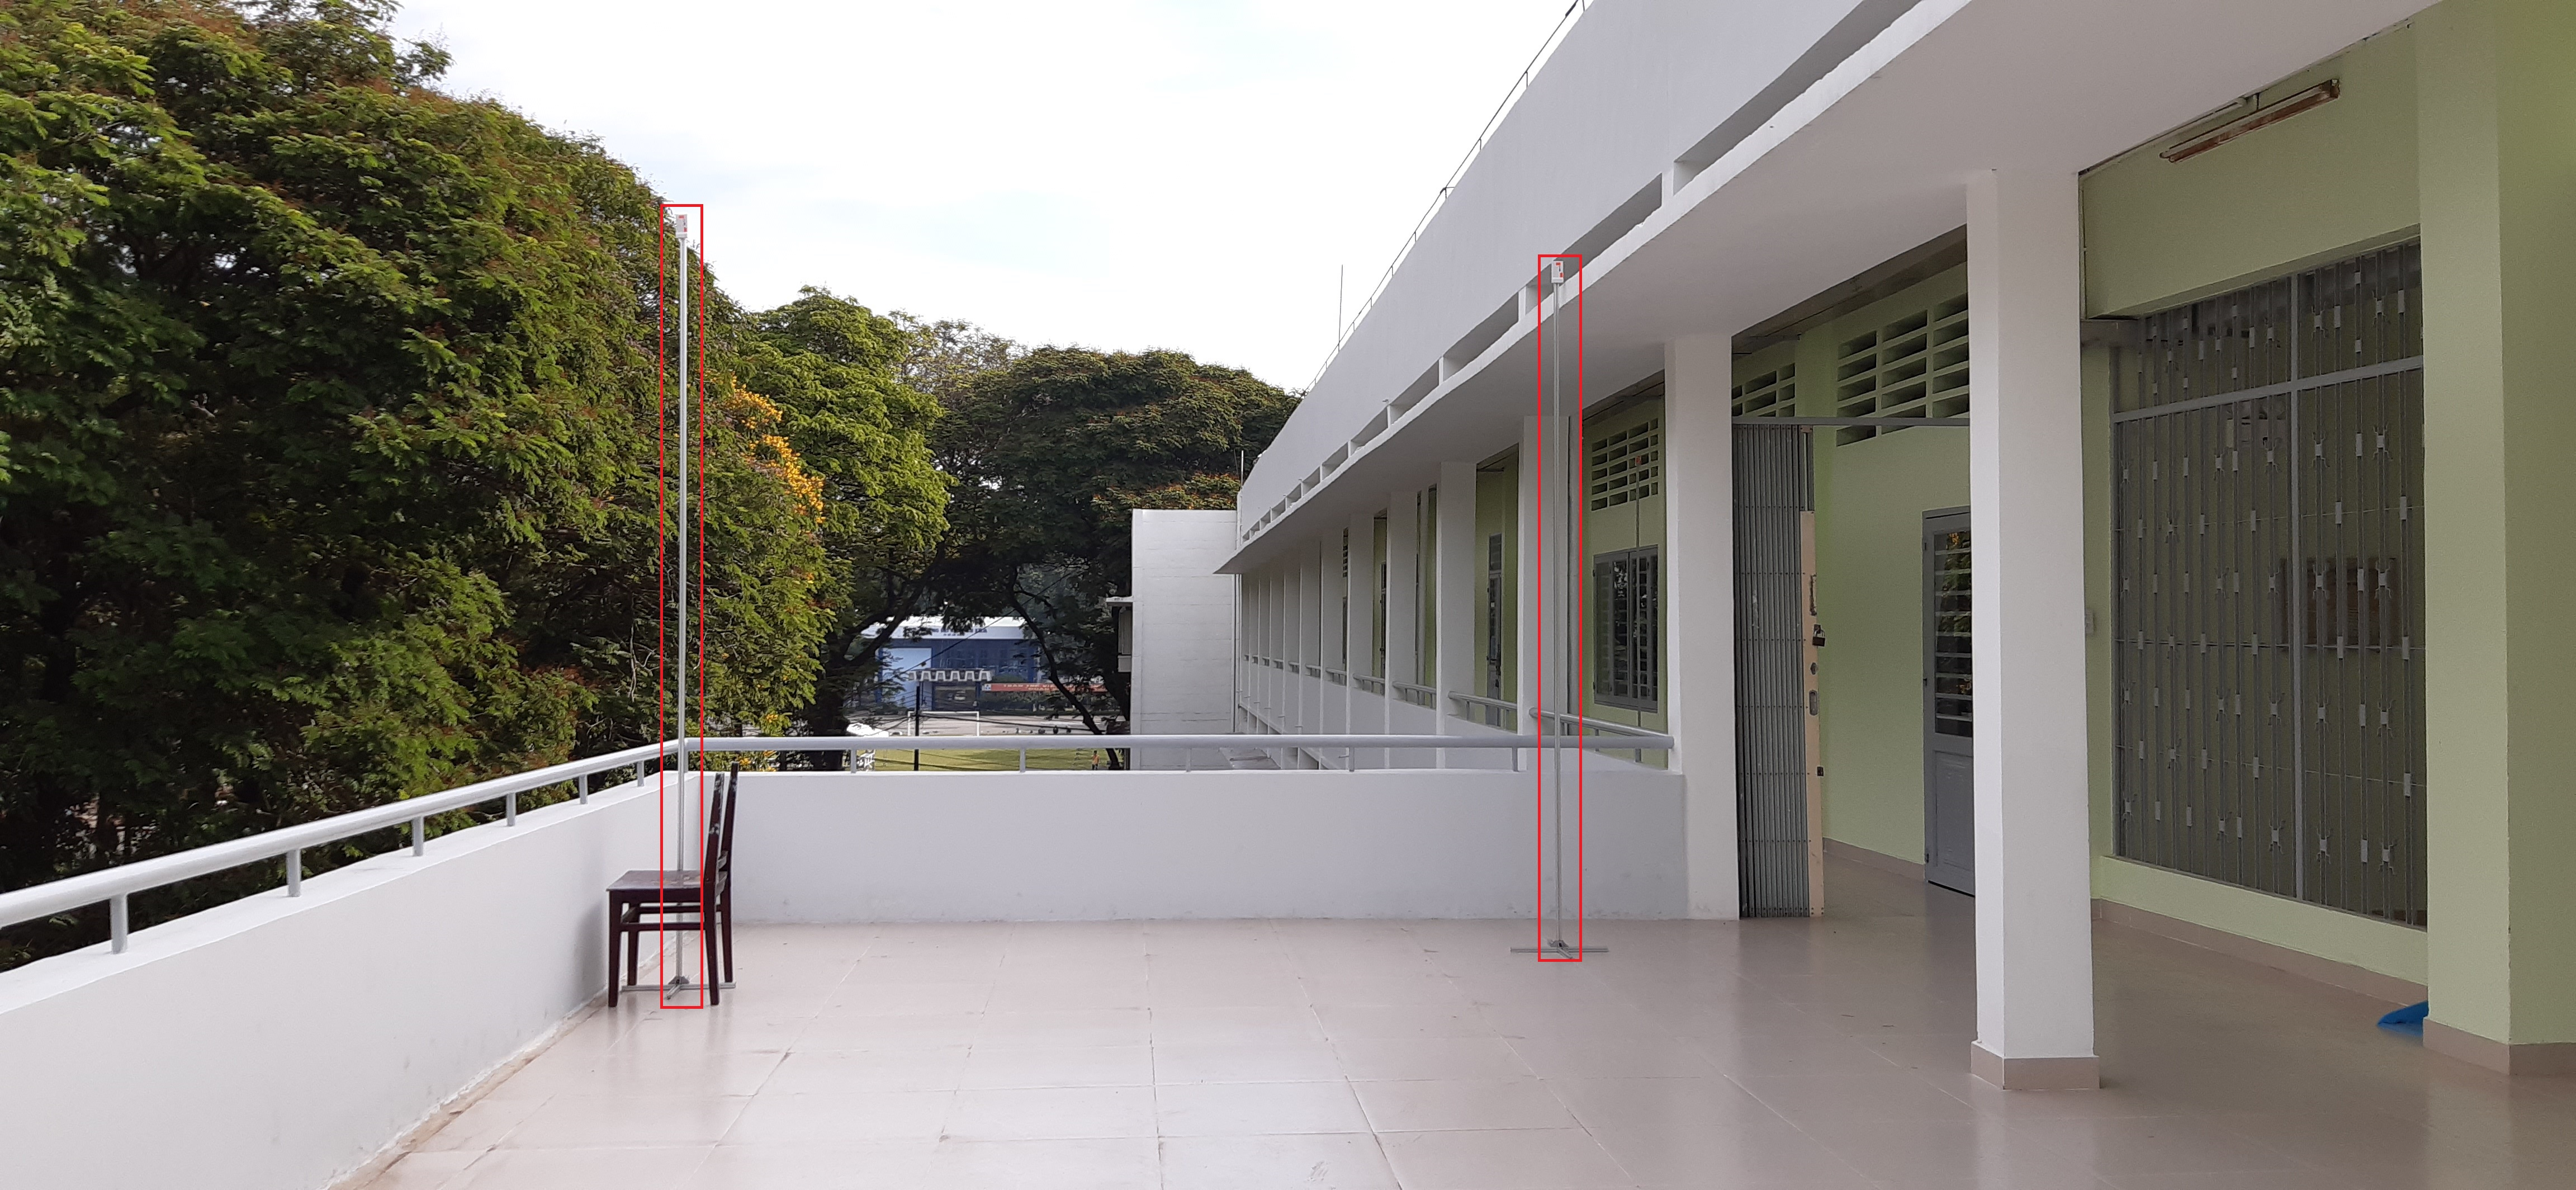
\includegraphics[width=1\textwidth]{arena_02.jpg}
    \caption{Node 2,3}
    \label{fig:node_2_3}
\end{figure}

% \begin{figure}[H]
%     \centering
%     \begin{subfigure}[b]{0.4\linewidth}
%         \centering
%         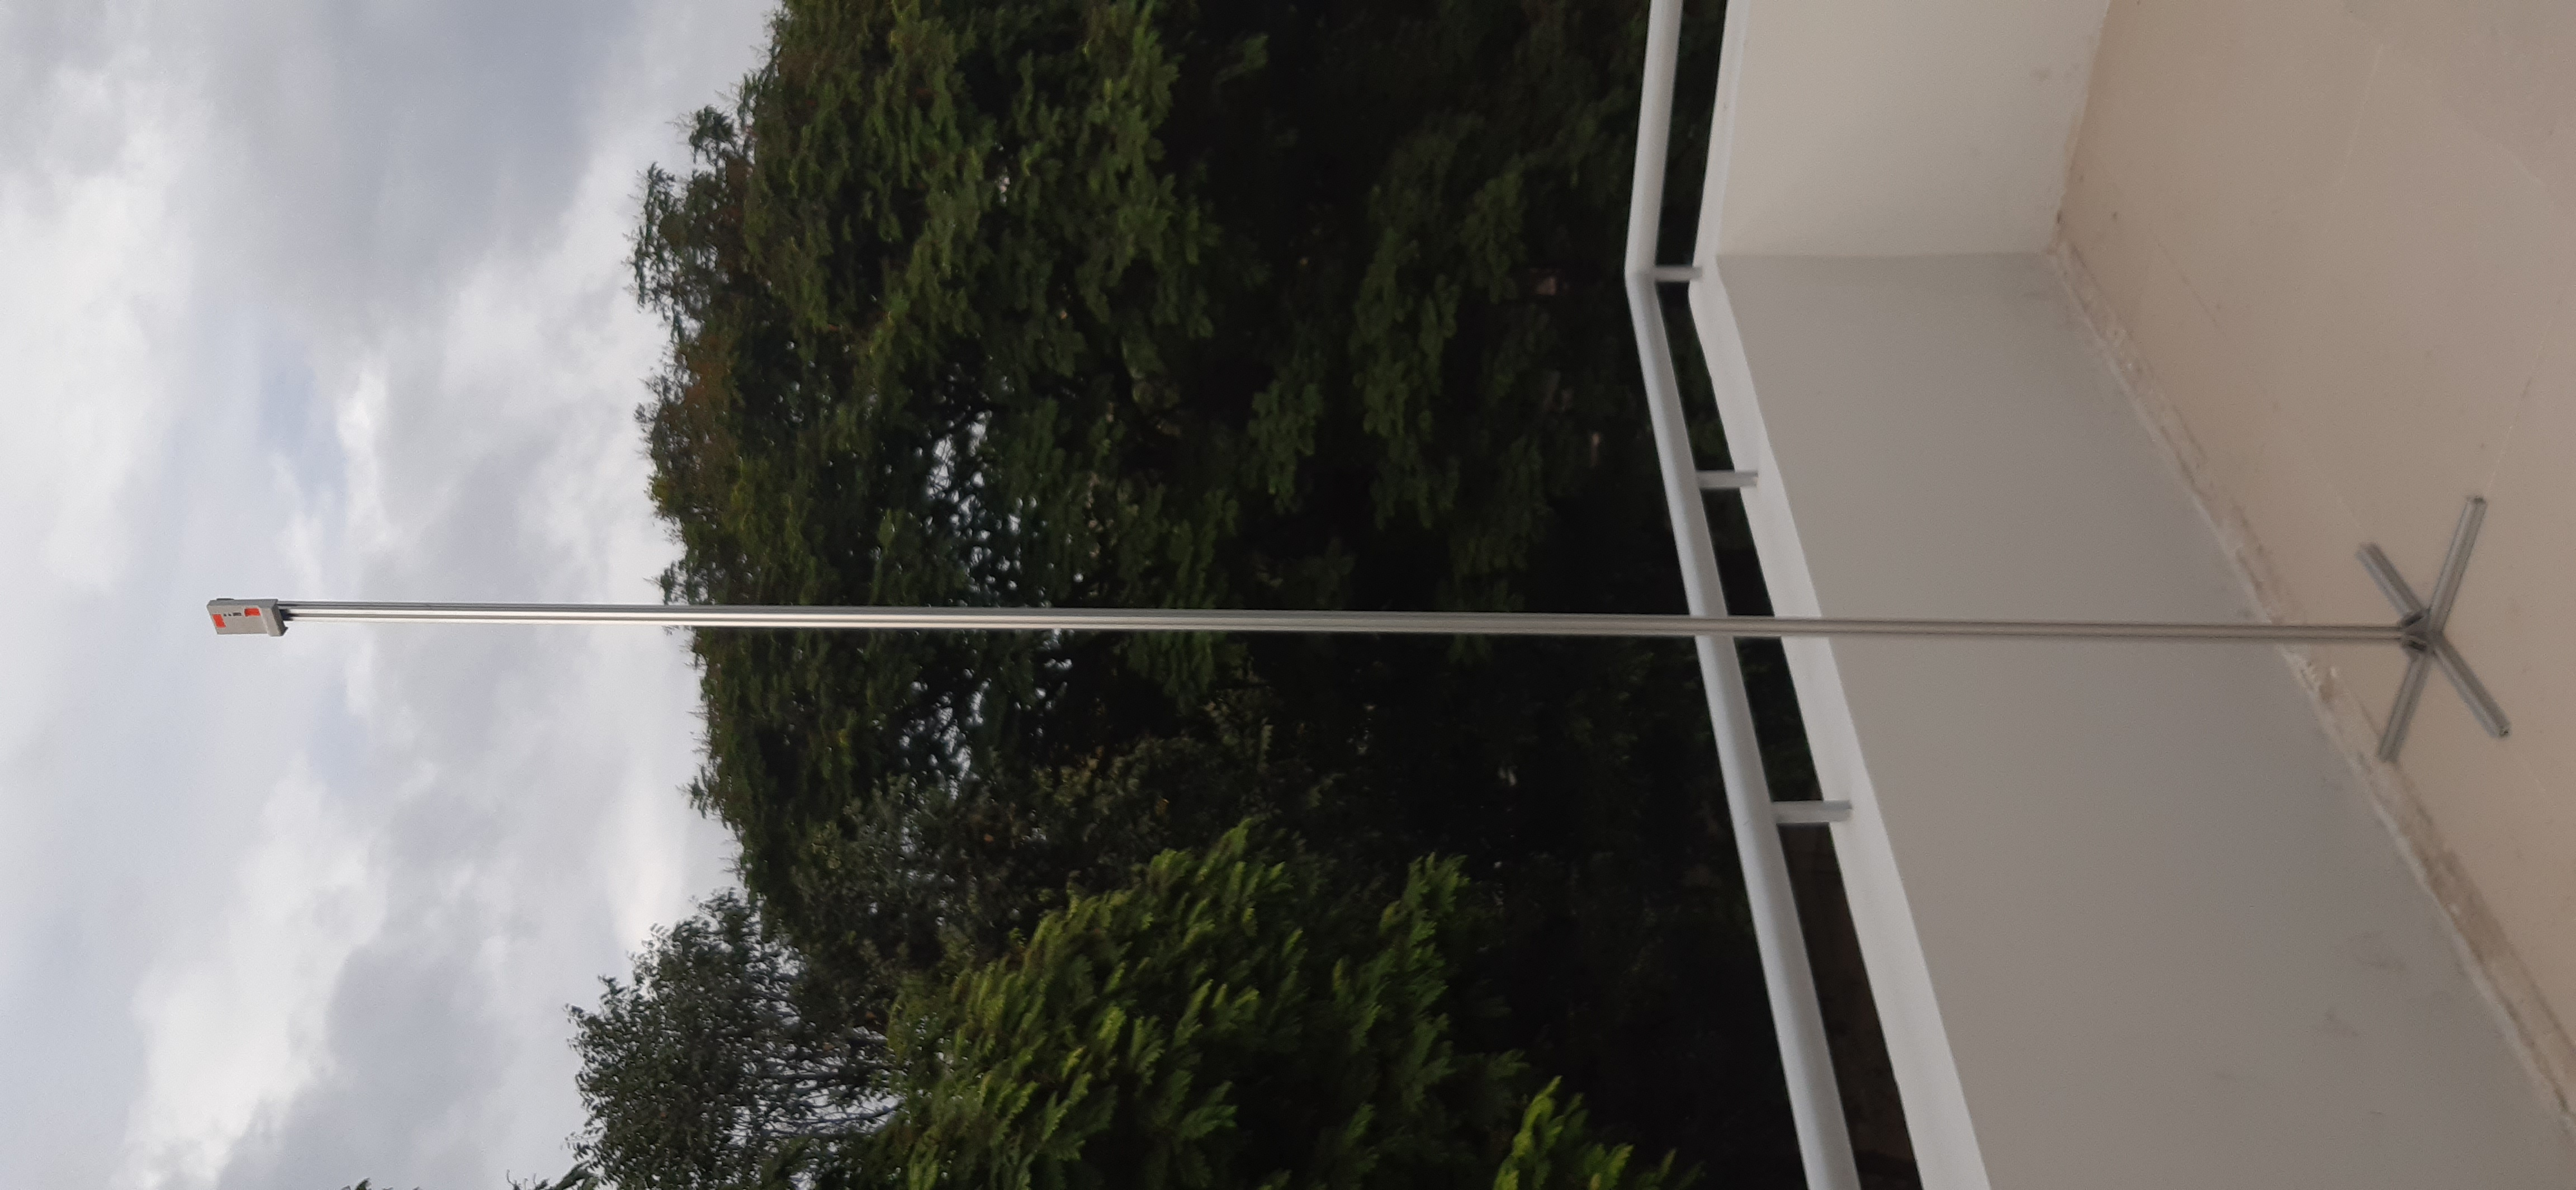
\includegraphics[angle=-90, width=0.65\linewidth]{arena_01.jpg}
%         \label{fig:arena_00}
%     \end{subfigure}
%     \begin{subfigure}[b]{0.4\linewidth}
%         \centering
%         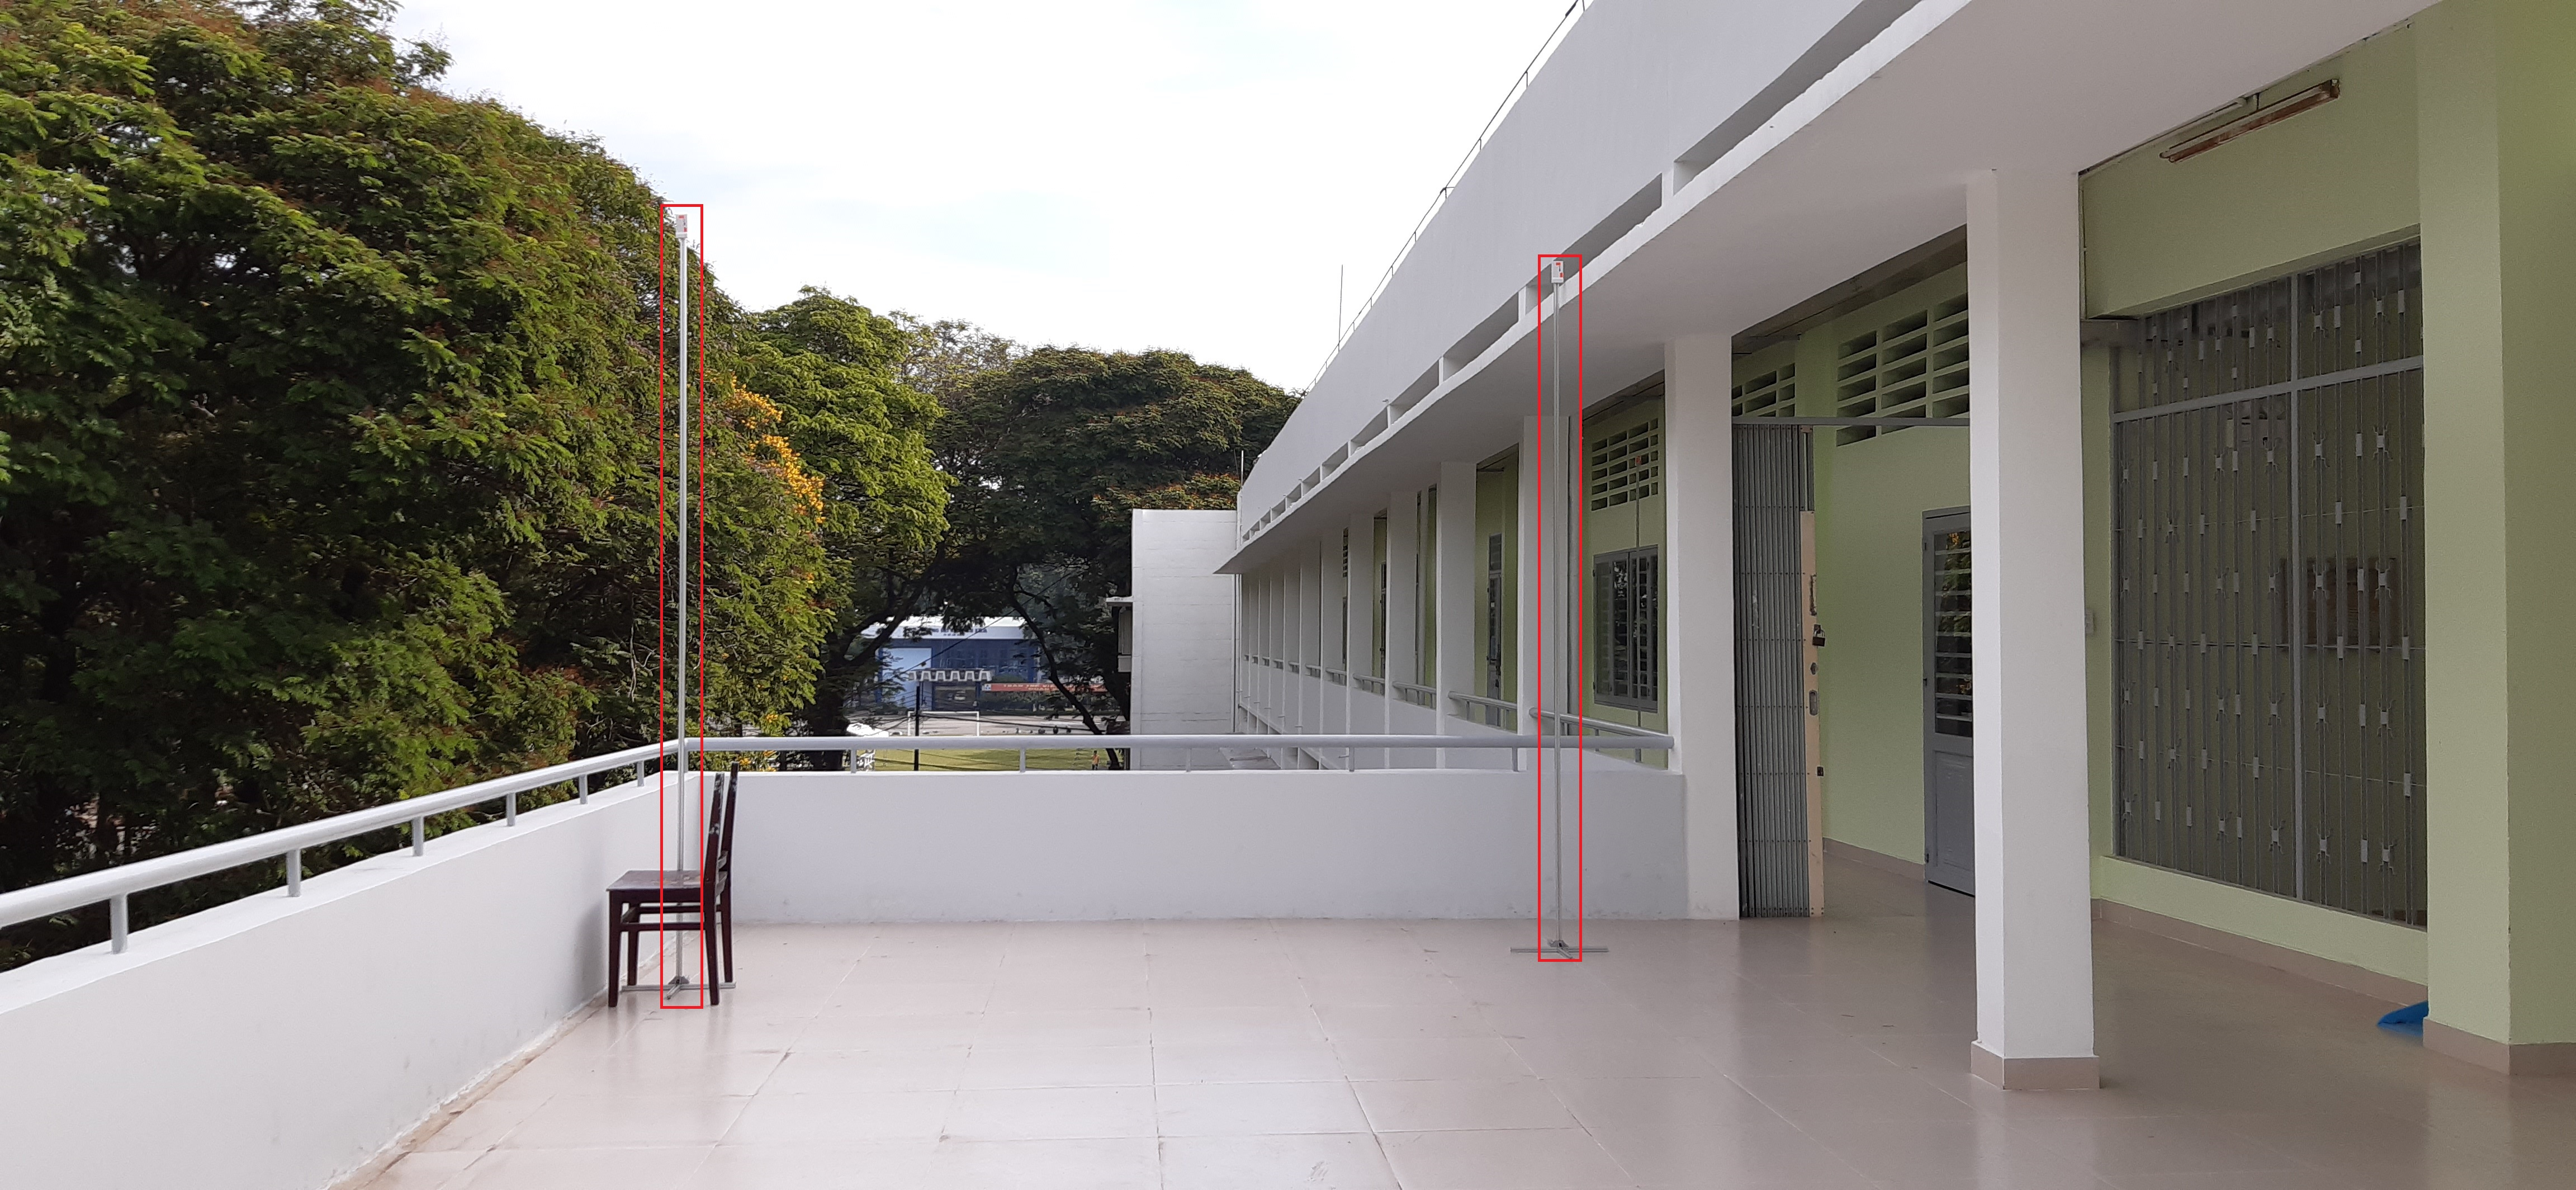
\includegraphics[angle=-90, width=0.65\linewidth]{arena_02.jpg}
%         \label{fig:arena_02}
%     \end{subfigure}
%     \caption{Node 3,4}
%     \label{fig:node_3_4_sep}
% \end{figure}

\begin{figure}[H]      
    \centering
    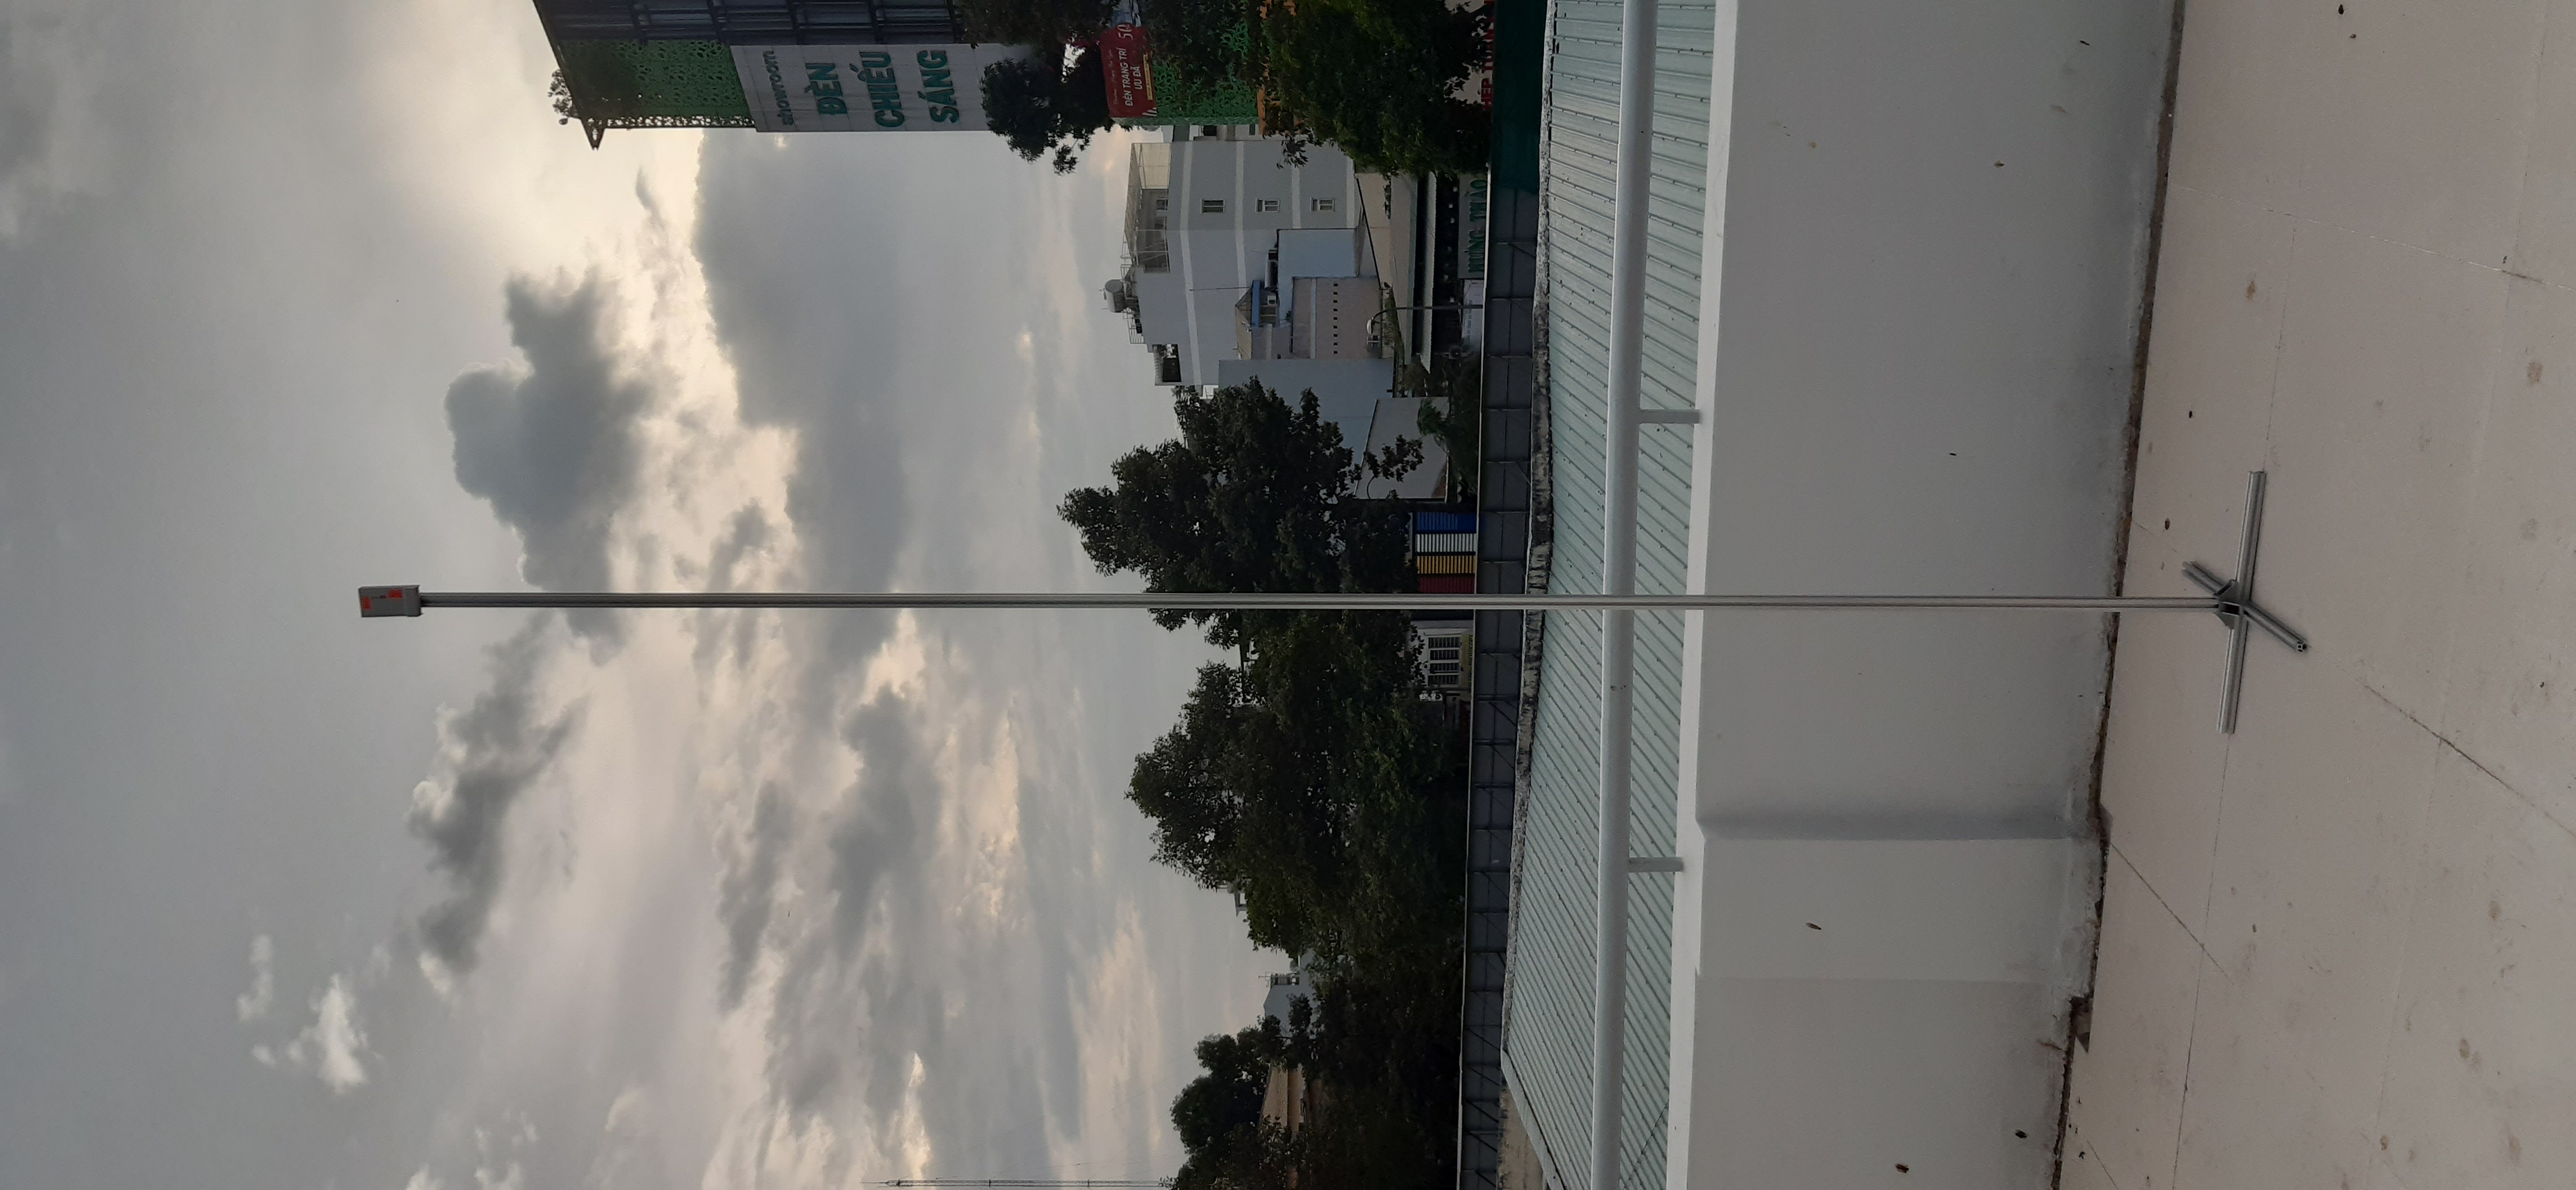
\includegraphics[width=1\textwidth]{arena_03.jpg}
    \caption{Node 4,5,6,7}
    \label{fig:node_4_5_6_7}
\end{figure}

The control and management interface for the experiment is shown in figure \ref{fig:proposed_rms_error}.
\begin{figure}[H]   
    \centering
    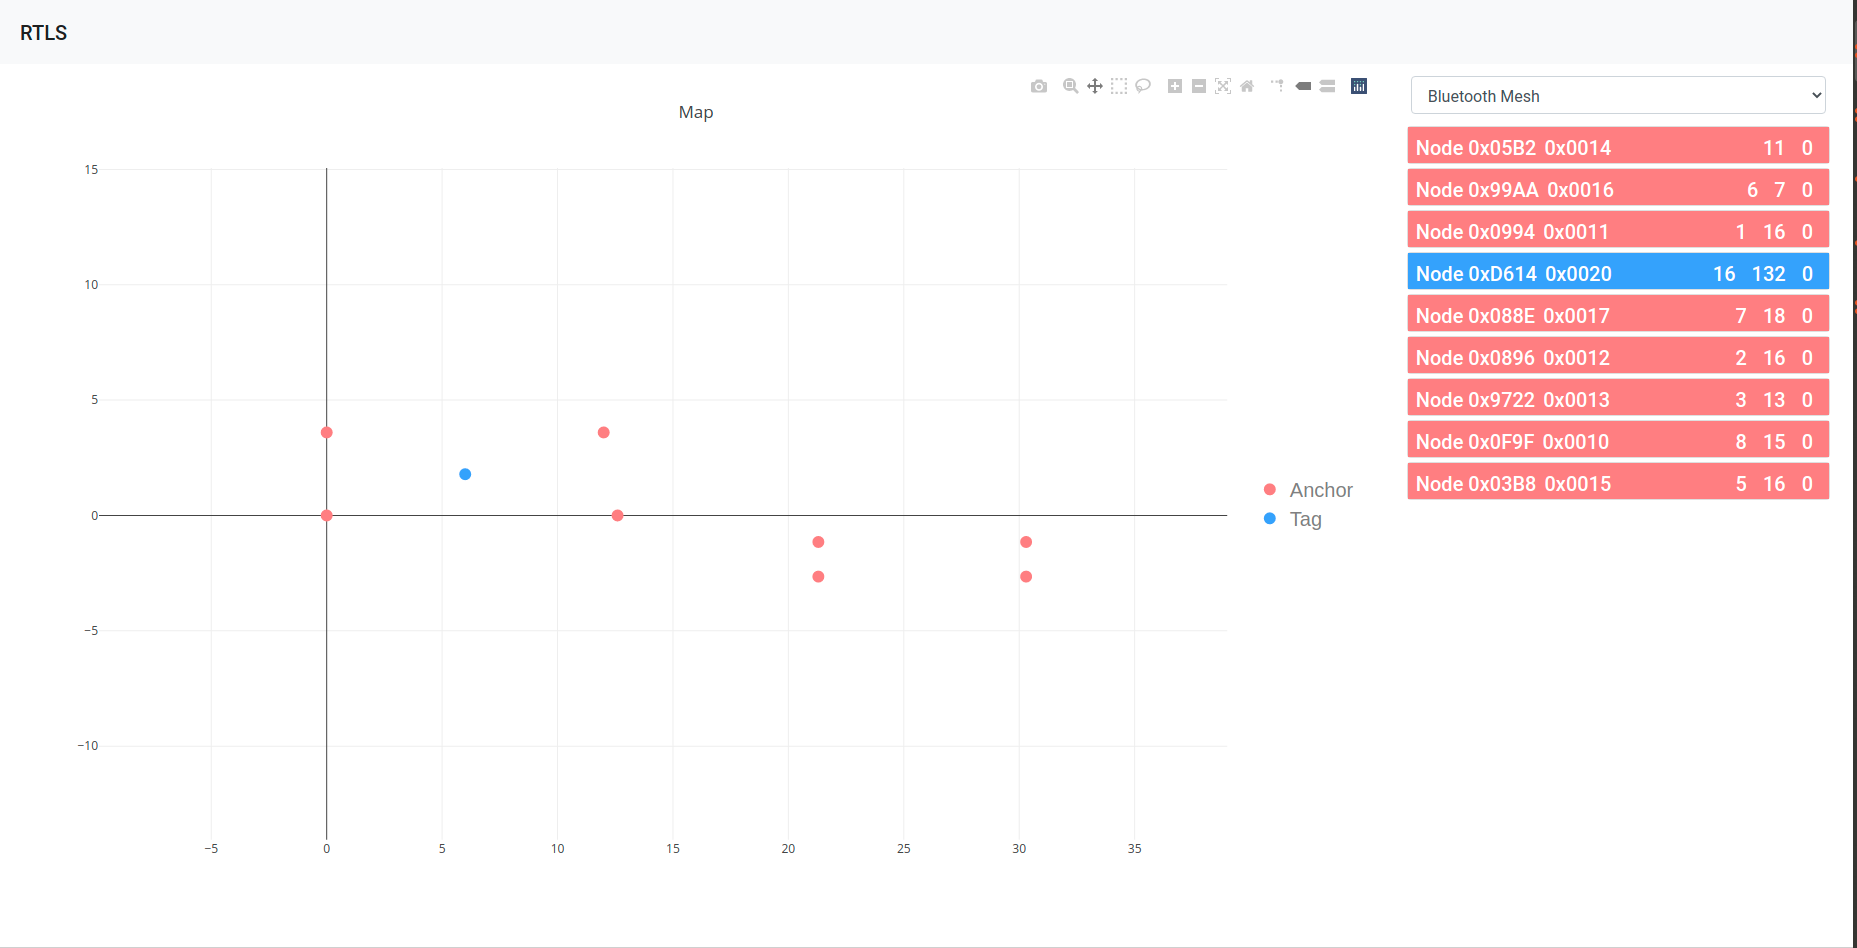
\includegraphics[width=1\textwidth]{result_gui.png}
    \caption{Indoor localization system GUI}
    \label{fig:result_gui}
\end{figure}

\subsection{Static result}
In this section, all results are obtained by statically placing tags in a fixed position and measuring the location. Moreover, all experiments are done with $z=3$.

Table \ref{table:vendor_rms_error} provides RMS errors of the vendor reference system relative to the position $(x,y)$. These errors are also graphically illustrated in \ref{fig:vendor_rms_error}.

Table \ref{table:proposed_rms_error} provides RMS errors of the proposed system relative to the position $(x,y)$. These errors are also graphically illustrated in \ref{fig:proposed_rms_error}.

\begin{table}[ht]
    \centering
    \begin{tabular}{|c|>{\centering\arraybackslash}p{2cm}|>{\centering\arraybackslash}p{2cm}|>{\centering\arraybackslash}p{2cm}|}
    \hline
    \backslashbox{y(m)}{x(m)}  &  3 & 7 & 10 \\ \hline
    0 &  0.2 &  0.28 &  0.25  \\ \hline
    2 &  0.14 &  0.13 &  0.18  \\ \hline
    4 &  0.22 &  0.19 &  0.27  \\ \hline
    \end{tabular}
    \caption{Vendor system error}
    \label{table:vendor_rms_error}
\end{table}

\begin{table}[H]
    \centering
    \begin{tabular}{|c|>{\centering\arraybackslash}p{2cm}|>{\centering\arraybackslash}p{2cm}|>{\centering\arraybackslash}p{2cm}|>{\centering\arraybackslash}p{2cm}|}
    \hline
    \backslashbox{y(m)}{x(m)}  &  1.2 & 4.8 & 9.6 & 10.8 \\ \hline
    0.6 &  0.10 & 0.20&  0.13 &  0.12  \\ \hline
    1.2 &  0.13 & 0.18&  0.17 &  0.16  \\ \hline
    2.4 &  0.09 & 0.10&  0.11 &  0.22  \\ \hline
    \end{tabular}
    \caption{Proposed system error}
    \label{table:proposed_rms_error}
\end{table}

\begin{figure}[H]
    \begin{minipage}[t]{\textwidth}       
        \centering
        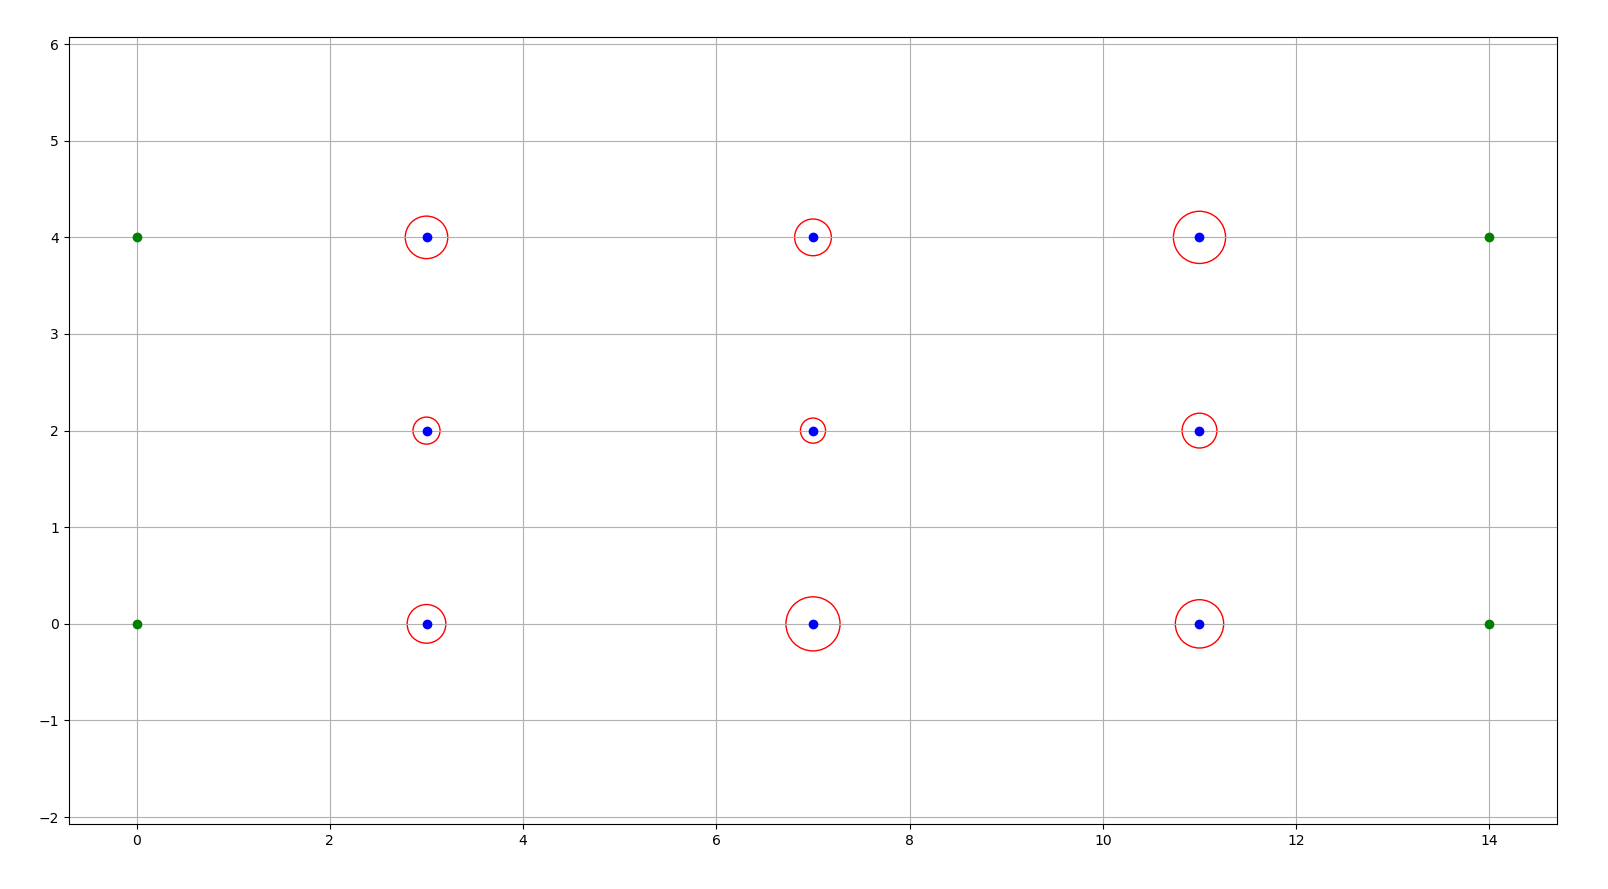
\includegraphics[width=1\textwidth]{rms_error}
    \end{minipage}
    \caption{Vendor system static error}
    \label{fig:vendor_rms_error}
\end{figure}

\begin{figure}[H]     
    \centering
    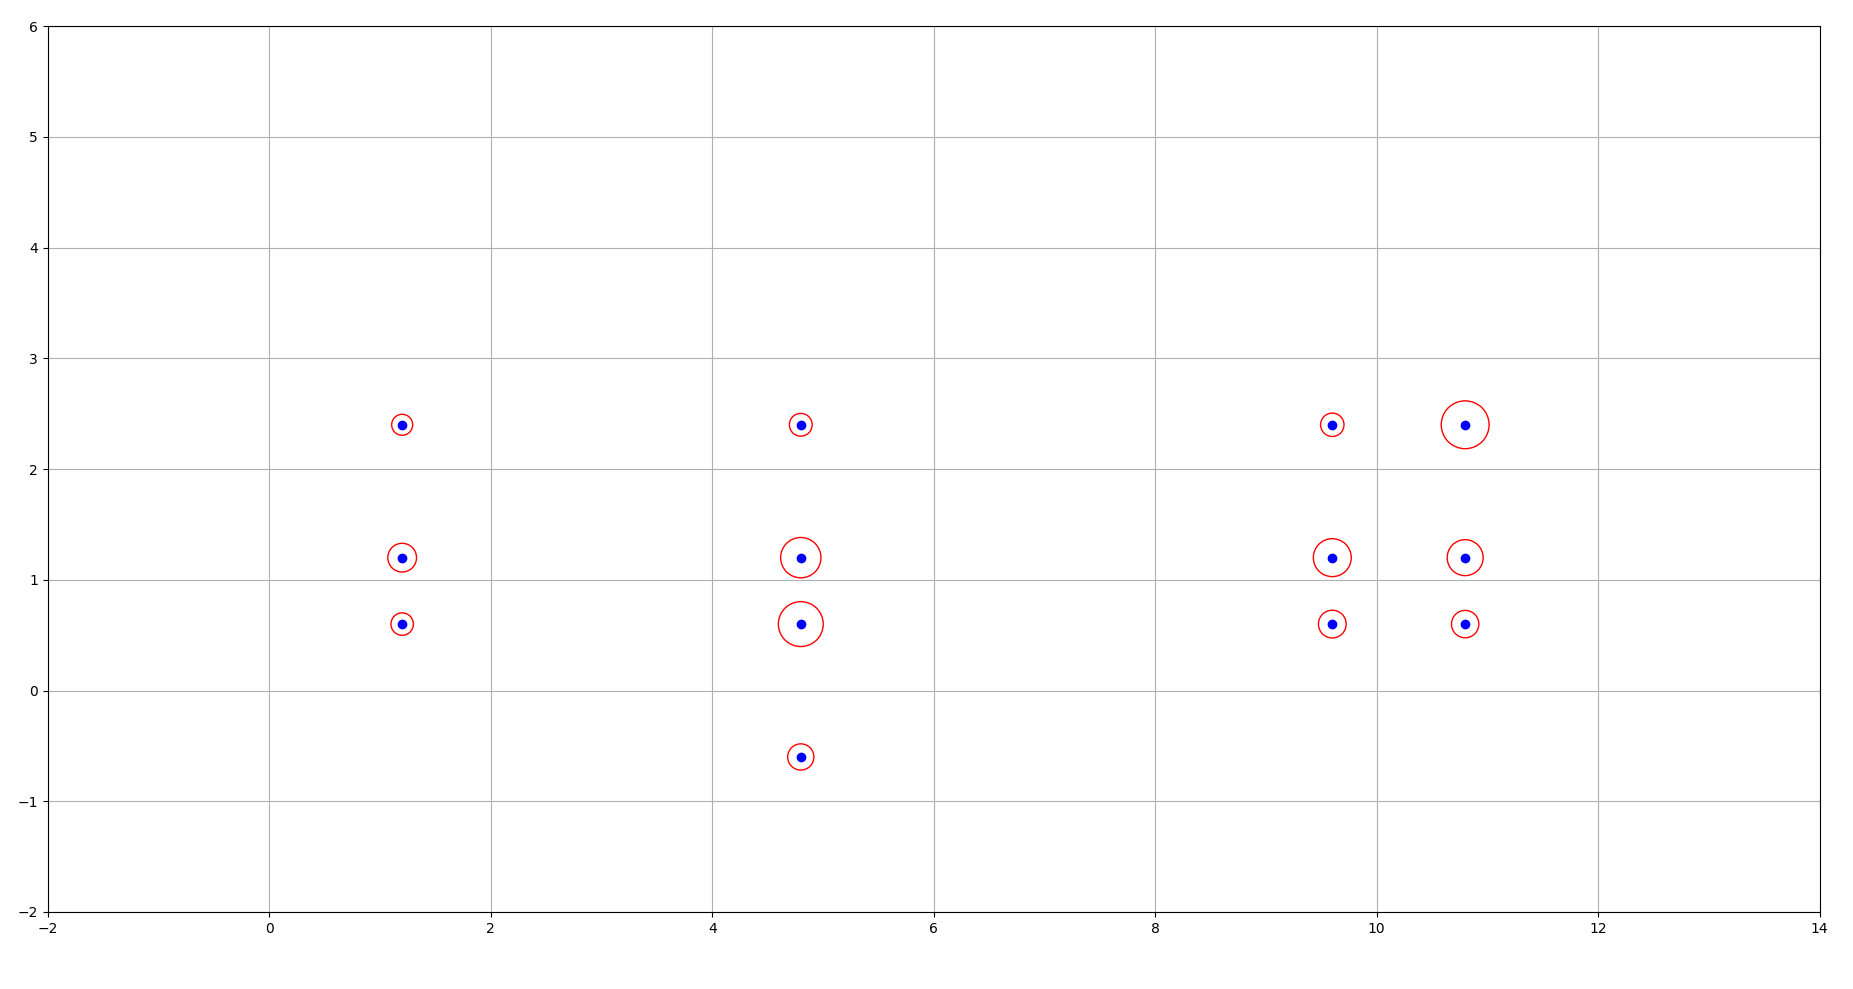
\includegraphics[width=1\textwidth]{result_static.png}
    \caption{Proposed system static error}
    \label{fig:proposed_rms_error}
\end{figure}

\subsection{Square movement result}
In this section, results shown in figure \ref{fig:result_square} are obtained as a tag moves along the boundary of a square. Since the reference path is not accurate enough, a numeric error is not provided. The only purpose is to give an intuitive performance evaluation of the system.
\begin{figure}[H]
    \centering
    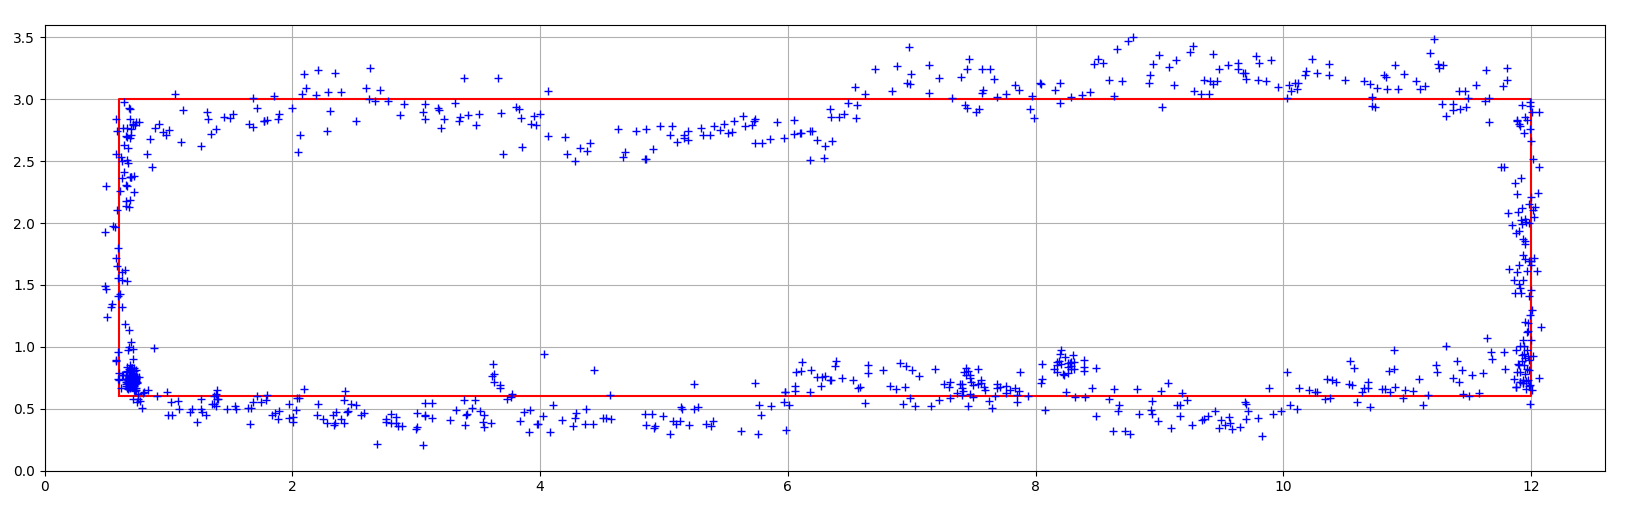
\includegraphics[width=1\textwidth]{result_square.png}
    \caption{Square movement result}
    \label{fig:result_square}
\end{figure}

\subsection{Multi-cell movement result}
In this section, results illustrated in figure \ref{fig:multi_cell_movement_result} are obtained as a tag moves along the red line. Since the reference path is not accurate enough, a numeric error is not provided. The only purpose is to give an intuitive performance evaluation of the system.
\begin{figure}[H]
    \centering
    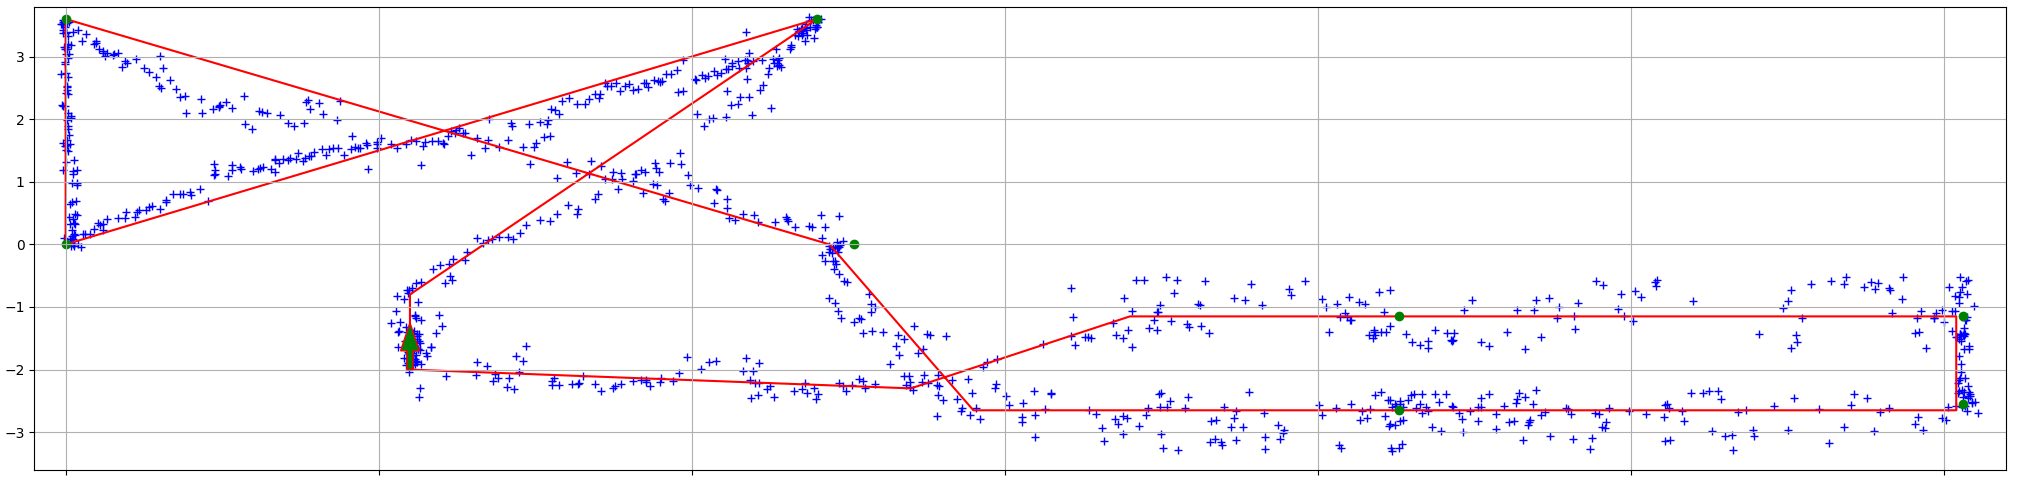
\includegraphics[width=1\textwidth]{path.png}
    \caption{Multi-cell movement result}
    \label{fig:multi_cell_movement_result}
\end{figure}

\subsection{Conclusion}
Using experimental results obtained from a decimeter-accuracy 3D indoor localization system, we conclude that the proposed system has a similar performance to the reference system given by the DecaWave while provides a better IoT service (Bluetooth mesh instead of normal Bluetooth Low Energy) which reduce the price of the entire system.

For a mobile tag, the system performance is relatively low but may acceptable for simple applications. Moreover, system error also increases significantly when anchors are placed to form a narrow shape. Hence, square topology should be used in practice.
\end{document}